\chapter{面向用户级QoS保障的接入网切片生成式资源预留与跨层优化机制}
\label{chap:resource}

\section{引言}

沿“感知—接入—资源分配—传输”的端到端传输链路，第~\ref{chap:perception}~章构建了退化遥测条件下可信的本地多跳状态感知，第~\ref{chap:handover}~章保障了海量终端接入的连续性与公平性。然而，稳定接入只是端到端服务质量（QoS）保障的起点：终端接入后，卫星仍须在受限的星上带宽与发射功率下为异构业务分配无线资源，才能将链路连接质量转化为用户级 QoS 满足。由此，本章从“接入”推进至“资源分配”，研究星上分布式管控范式下面向资源使用效率与用户级 QoS 联合保障的切片--MAC 跨层无线资源分配方法。

在已接入用户承载异构业务的 LEO 卫星接入网（LEO satellite Radio Access Network，LEO-sRAN）中，单颗卫星可用的带宽与发射功率十分有限，资源预算必须转化为用户级 QoS 满足，而不是单纯提高聚合吞吐。其根本困难在于切片层预算与 MAC 层执行之间存在跨时隙滞后：一次切片层资源预算须经后续多个媒体接入控制（MAC）时隙中的业务到达、信道变化与流级竞争之后，才反映为用户级 QoS 是否满足。更关键的是，聚合吞吐并不等价于用户级 QoS。如图~\ref{fig:ch4_pf_scheduling}~所示，即便聚合传输速率超过名义门限，随业务流密度上升仍有部分应用流违背各自的速率--时延要求。因此，LEO-sRAN 资源分配必须显式考量个体业务流的 QoS 可满足能力，而非仅依据聚合吞吐~\cite{sui-ConvexOptDLResAlloc-TCCN24}。

\begin{figure}[!htp]
    \centering
    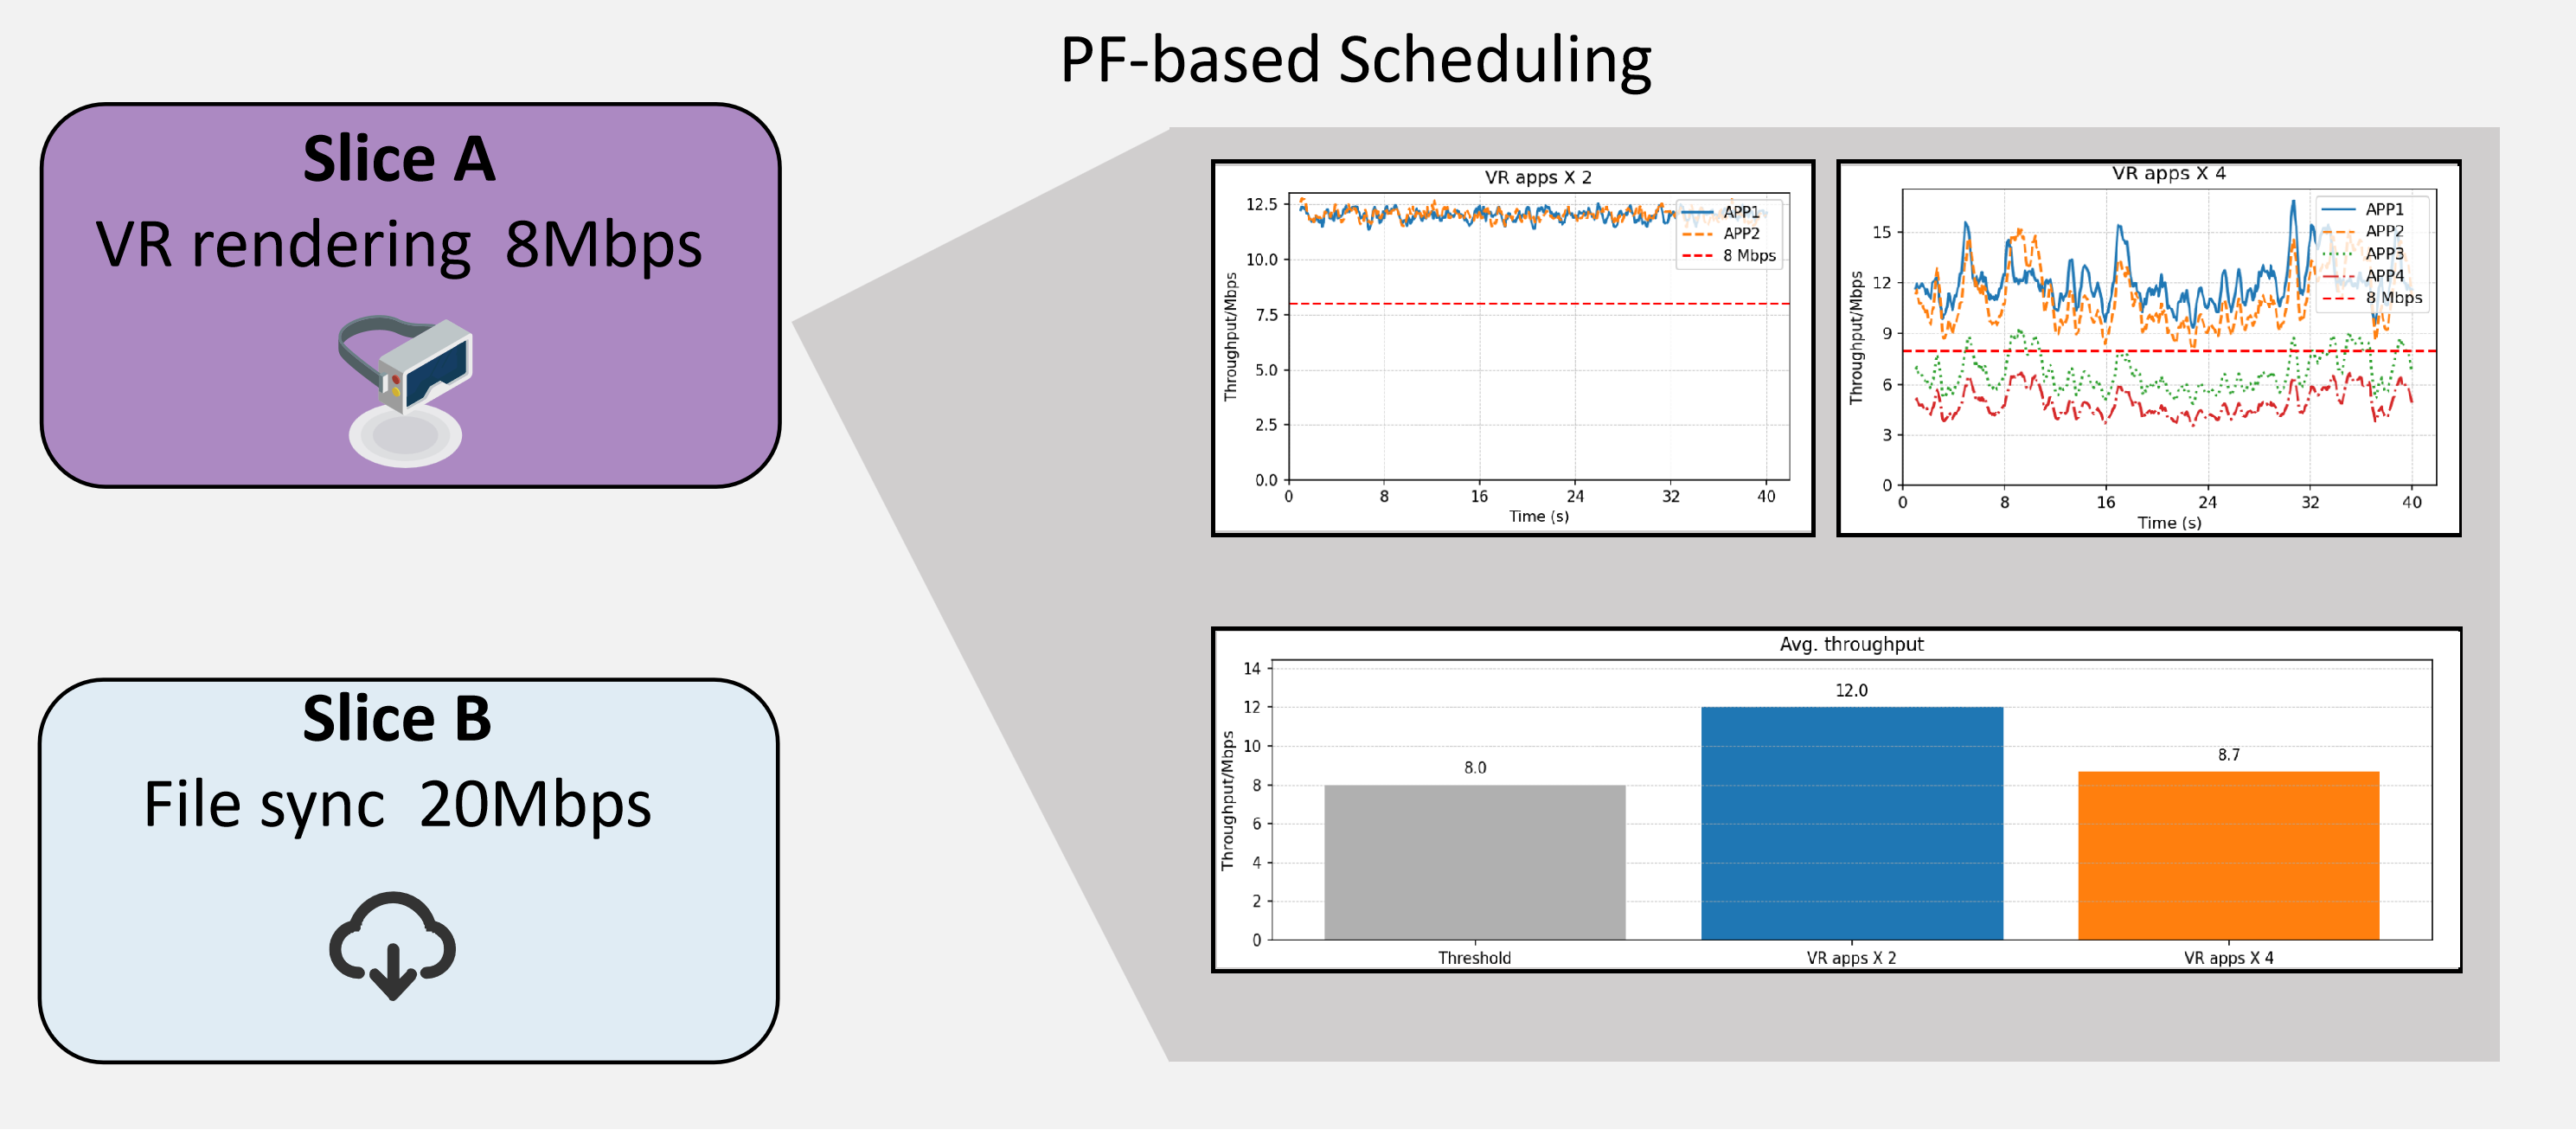
\includegraphics[width=0.82\linewidth]{figures/chapter4/Fig1_PF_scheduling.png}
    \caption{业务流密度上升时聚合传输速率与用户级 QoS 满足之间的失配现象}
    \label{fig:ch4_pf_scheduling}
\end{figure}

无线接入网切片（Radio Access Network Slicing，RAN Slicing）将 QoS 需求相近的业务归并为逻辑切片并在切片层预留带宽与功率~\cite{li-HierarchicalSoftRANSlicing-WirelessComms20}，为差异化业务保障提供了可部署的资源组织方式，但切片--MAC 分层也在粗粒度预算与用户级 QoS 满足之间引入了可满足能力缺口：切片层多预测业务需求或依据已实现性能调整预算，未刻画当前预算经 MAC 层竞争与信道变化后如何影响未来用户级 QoS；MAC 层则以队列紧迫度尽力而为地调度，不判定当前预算下速率--时延门限是否可满足。这构成一个跨时间尺度的资源协同问题：切片层须预测由当前预算到未来用户级 QoS 满足能力的映射，MAC 层须将预算转化为 QoS 可行的时隙级业务流调度。

然而，现有研究尚未将这一跨时间尺度的 QoS 映射贯通：切片层资源配置仍以业务需求预测或已实现性能反馈为依据~\cite{liu-reconfigurableRanSlicing-TCCN25,chen-InfoRanSlicing-JSAC24,Phyu-MultiSlicePrivacy-TNSM23}，MAC 层调度仍以聚合吞吐、队列稳定性或积压紧迫度为准则~\cite{leng-SchedulingResourceSat-ChinaCom22,Villegas-OptimizingQoS-TNSM26}，二者均未判定业务流的 QoS 门限在当前预算下是否可满足。这种相互割裂的反应式调度无法形成切片--MAC 跨层协同，难以适应 LEO 卫星网络的高动态性。因此，仍缺乏一种能够预测当前预算对用户级 QoS 满足能力的影响、并将其转化为可执行 MAC 调度的切片--MAC 协同机制。

针对上述问题，本章提出面向 LEO-sRAN 的双时间尺度预测调度（Dual-Timescale Predictive Scheduling，DTPS）框架，以带宽与功率预算为跨层接口、以用户级 QoS 满足能力为切片层与 MAC 层协同准则，将长期 QoS 保障分解为切片层的预测式资源预留与 MAC 层的时隙级业务流调度：切片层预测当前预算能否支撑未来用户级 QoS，并以预算界定 MAC 层调度的可行域；MAC 层在该可行域内优先调度 QoS 门限可满足且 QCI/5QI 优先级较高的业务流，使有限带宽与功率优先转化为有效 QoS 收益而非单纯聚合吞吐。具体而言，切片层采用反馈校正的业务--信道演化预测模型，生成候选资源预算下的用户级 QoS 预测演化轨迹，从而在预算决策前评估不同资源配置对长期 QoS 满足率的支撑能力；MAC 层则估计候选业务流满足速率--时延门限所需的最小资源块组（Resource Block Group，RBG）和功率开销，仅纳入 QoS 可行流，并依据 QCI/5QI 优先级在固定切片预算内完成业务流选择与资源映射。

本章的主要贡献总结如下：
\begin{itemize}
\item 将资源高效的用户级 QoS 保障建模为随机业务到达与时变服务能力下的双时间尺度切片--MAC 资源分配问题，并以带宽与功率预算为跨层接口，将切片级资源预留与时隙级业务流调度相衔接，使切片层负责维持长期 QoS 可满足能力，MAC 层负责在固定预算内执行 QoS 可行的业务流选择。

\item 针对切片层难以前瞻评估预算效果的问题，提出生成式切片资源预留机制，即能够生成候选资源预算长期 QoS 演化的预测式资源预留机制。该机制通过反馈校正的业务--信道演化预测模型，刻画业务到达、信道服务能力和队列状态在不同预算下的演化规律，而非仅预测业务需求；利用 MAC 层反馈校正预测轨迹，使切片层能够在预算决策前评估候选资源配置对长期 QoS 满足率的影响。

\item 针对 MAC 层难以判断当前预算下 QoS 门限是否可满足的问题，提出 QCI/5QI 优先级感知的 QoS 可行流调度器，将候选业务流满足速率--时延门限所需的最小 RBG--功率开销作为准入依据，并在切片预算下优先选择业务优先级高且 QoS 可行的业务流。

\item 在 Starlink 规模星座上的仿真表明，DTPS 在过载业务和突发业务增强条件下均能保持较高的用户级 QoS 满足率，并在资源消耗与平均时延之间取得稳定折中；消融与固定预算调度对比进一步验证了切片层预测式资源预留和 MAC 层 QoS 可行性测试的作用。
\end{itemize}

\section{系统模型与问题建模}
\label{sec:ch4_sysmodel}

本节在第~\ref{sec:dist-arch}~节确立的纯分布式管控范式下，对单颗 LEO 卫星的下行无线资源管理过程建模。在该范式下，卫星不依赖核心网集中调度，而是依据本地切片级业务统计与有限邻星上下文，在慢时间尺度上自主完成切片资源预留、在快时间尺度上完成时隙级用户调度。下文依次建立网络与切片架构模型、无线资源分配模型、业务与 QoS 效用模型以及星地链路与时延模型，并在此基础上将面向用户级 QoS 保障的无线资源管理形式化为长期资源消耗最小化问题。全章符号含义参见文前的主要符号对照表。

\subsection{网络与切片架构模型}
\label{subsec:ch4_network}

如图~\ref{fig:ch4_system_model}~所示，考虑一个 LEO 卫星接入网为某一地理区域提供下行接入服务，该区域同时处于多颗 LEO 卫星的覆盖之下。每颗卫星采用多波束天线，以直连入网（Direct-to-Cell）方式为其覆盖范围内的地面终端提供接入。地面终端产生异构业务需求，既包含时延敏感型业务，也包含带宽密集型业务。为支撑差异化的 QoS 保障，这些业务按其主导 QoS 特征归并为两类逻辑切片：无线资源首先在切片层面进行预留以满足异构 QoS 需求，随后再经 MAC 层调度分配至各用户。

考虑到星地回程链路可能存在较长时延与间歇性可用~\cite{zhou-FeederLinkHandover-Sensors23}，下行无线资源管理在每颗卫星本地执行，而非依赖核心网集中控制；切片上下文仅在回程链路条件允许时机会式地上报核心网。可见卫星与波束间的同信道干扰假定已通过波束赋形传输调度与跳波束机制加以抑制~\cite{wang-CollinearInterference-TCOM25}，故不计入本章建模。在该架构下，LEO-sRAN 的资源分配由运行于不同时间尺度的两层决策构成：慢时间尺度的切片资源预留确定各切片预算，快时间尺度的 MAC 调度在该预算内将资源分配至用户。

\begin{figure}[!htp]
    \centering
    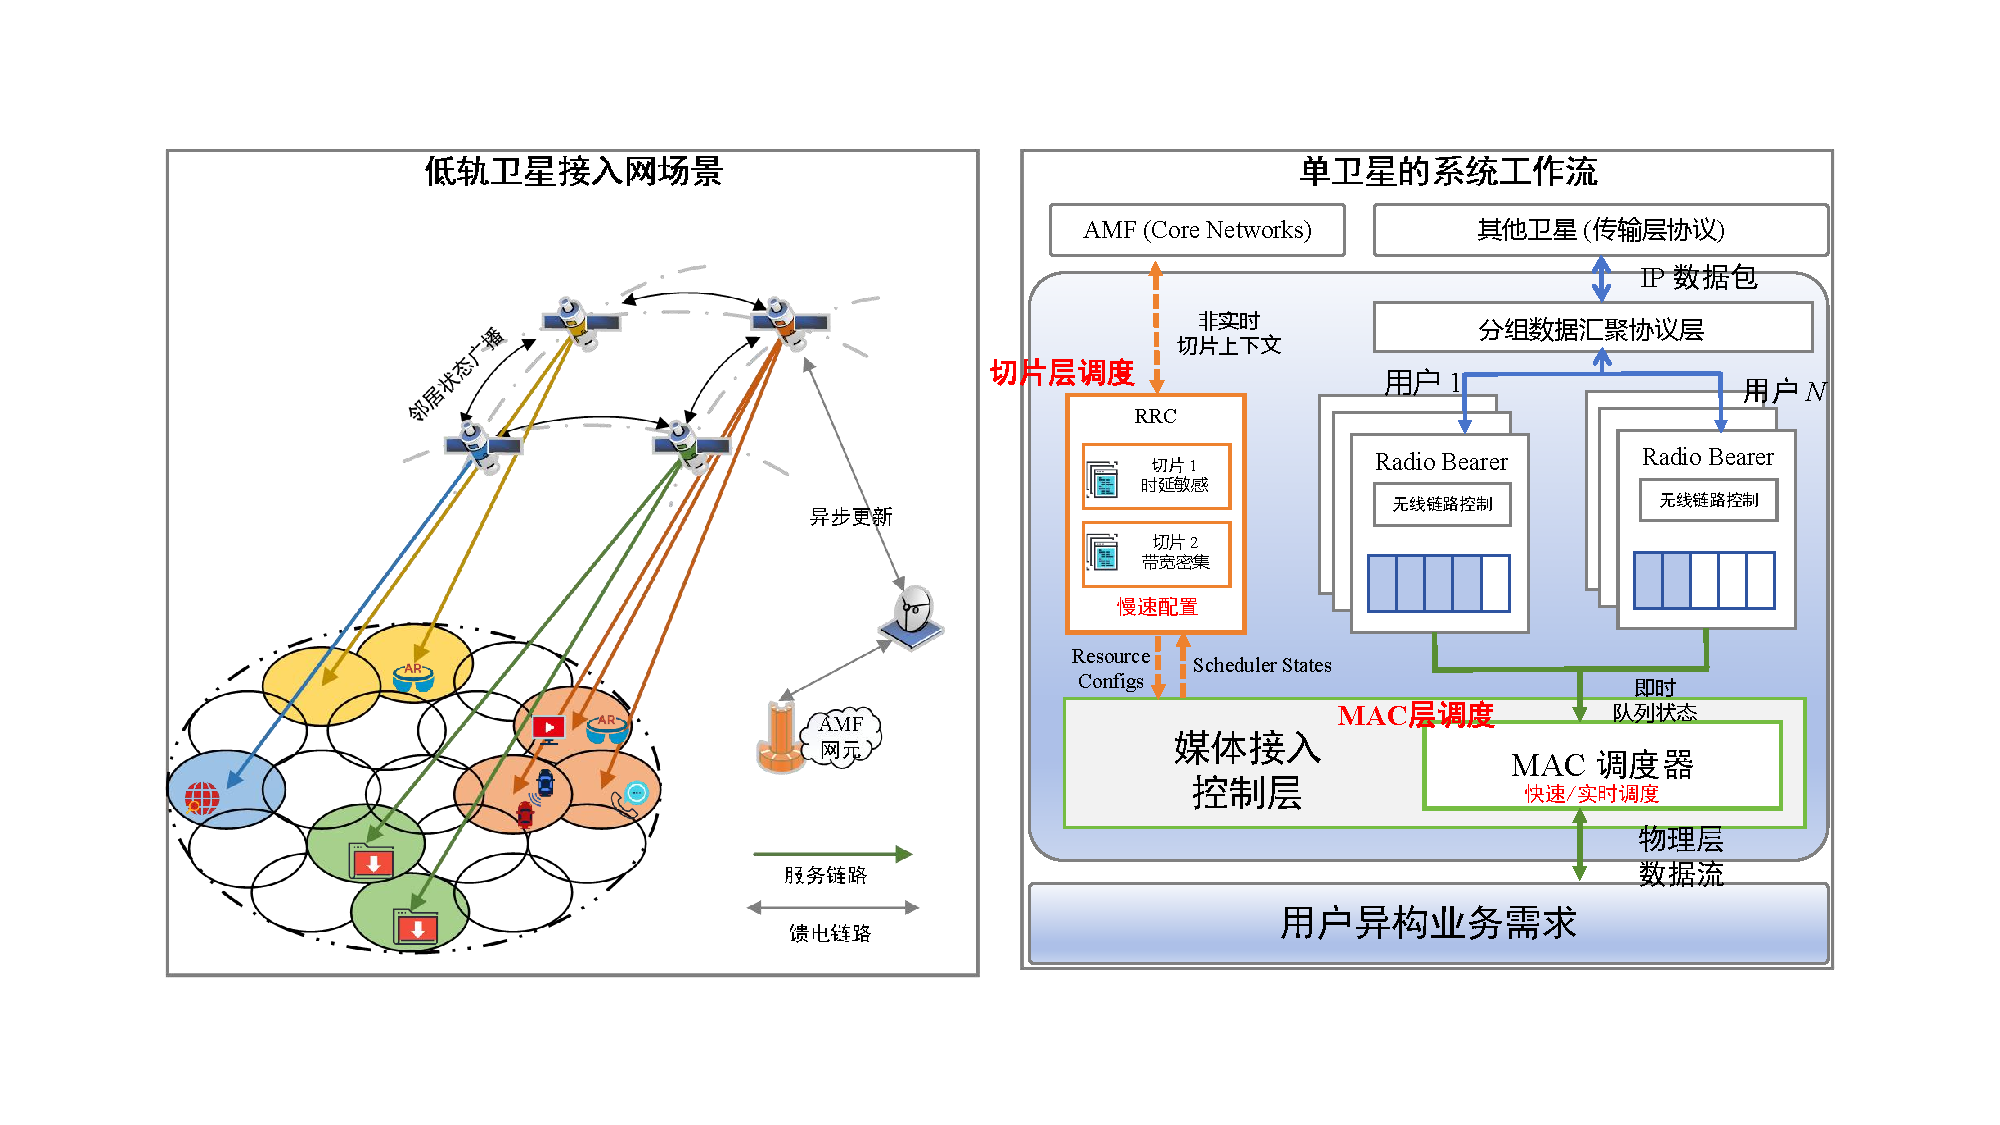
\includegraphics[width=0.82\linewidth]{figures/chapter4/Fig3_system-model.pdf}
    \caption{LEO 卫星接入网系统架构：左侧为多星覆盖与邻星状态交互的网络场景，右侧为单颗卫星内部的资源管理工作流}
    \label{fig:ch4_system_model}
\end{figure}

考虑卫星集合 $\mathcal S=\{1,\dots,S\}$ 在某一地理覆盖区域内为地面终端集合 $\mathcal U=\{1,\dots,U\}$ 提供下行接入。由于 LEO 卫星相对地面高速运动，地面终端在所考虑的时间范围内可近似视为静止。卫星以离散时隙运行，时隙为最小资源分配单元。记 $\mathcal T=\{1,\dots,H\}$ 为长度为 $H$ 个时隙的调度区间，在该观测区间内卫星集合 $\mathcal S$ 与目标区域之间的可见关系保持不变，因而可见卫星集合在观测区间内固定。

资源预留运行于较慢的切片时间尺度，记切片间隔索引为 $k$；MAC 调度运行于较快的时隙尺度。由于切片间隔时长 $T_s$ 远大于 MAC 时隙时长 $T_\text{MAC}$，每个切片间隔包含多个 MAC 时隙，记为 $\mathcal T_k\triangleq\{(k-1)N_\text{MAC}+1,\dots,kN_\text{MAC}\}$，其中 $N_\text{MAC}=T_s/T_\text{MAC}$。

初始时，每个终端接入其可见范围内距离最近的卫星，因较短的传播距离通常带来较强的接收信号。由于用户空间分布不均与业务需求异构，即便在同一覆盖区域内，不同卫星也可能承受失衡的业务负载。因此，用户关联在切片时间尺度上进行调整，通过联合考虑链路质量与卫星负载在可见卫星之间重分布业务。记 $\mathcal S_u\subseteq\mathcal S$ 为终端 $u$ 的可见卫星集合，$a_{u,s}(k)\in\{0,1\}$ 为切片间隔 $k$ 的关联指示：$a_{u,s}(k)=1$ 表示终端 $u$ 在间隔 $k$ 内由卫星 $s$ 服务，否则为 $0$。关联决策满足
\begin{equation}\label{eq:ch4_association}
\sum_{s\in\mathcal S_u}a_{u,s}(k)=1,\quad \forall u\in\mathcal U,\ k\ge1.
\end{equation}
卫星 $s$ 在间隔 $k$ 内服务的终端集合定义为 $\mathcal U_s(k)\triangleq\{u\in\mathcal U\mid a_{u,s}(k)=1\}$。

考虑到同一终端可同时承载多个 QoS 需求各异的逻辑应用，本章以应用流为资源分配与 QoS 保障的基本服务单元：地面终端产生的每个逻辑应用视为一条应用流，以 $i$ 索引，全体应用流集合记为 $\mathcal I$；终端仅作为应用流的物理载体，记 $u(i)\in\mathcal U$ 为承载流 $i$ 的终端。应用流经其载体终端的星地链路传输，其服务卫星随终端关联确定，卫星 $s$ 在间隔 $k$ 内服务的应用流集合为 $\mathcal I_s(k)\triangleq\{i\in\mathcal I\mid a_{u(i),s}(k)=1\}$。下文“业务流”均指此类应用流。

\subsection{无线资源分配模型}
\label{subsec:ch4_radio}

带宽与发射功率是 LEO-sRAN 的主要无线资源~\cite{Balasingam-RANSlicing-NSDI24}：发射功率用于补偿大尺度传播损耗，带宽则决定传输速率并直接影响时延。在每个时隙 $t\in\mathcal T$ 内，每颗卫星向其服务的业务流分配带宽与功率。下行传输采用正交频分多址（Orthogonal Frequency-Division Multiple Access，OFDMA）结构，与 Starlink 等现代 LEO 星座一致~\cite{Neinavaie-StarlinkSignal-TAES24}。记 $W_s$ 为卫星 $s$ 可用的下行总带宽，划分为若干正交资源块（RB）。实际调度器将连续 RB 聚合为资源块组（RBG）以降低调度复杂度，记卫星 $s$ 的 RBG 集合为 $\mathcal G_s=\{1,\dots,N_s^\text{RBG}\}$。引入 RBG 分配变量 $x_{i,s,g}(t)\in\{0,1\}$，$x_{i,s,g}(t)=1$ 表示卫星 $s$ 的 RBG $g\in\mathcal G_s$ 在时隙 $t$ 分配给业务流 $i$。由于每个 RBG 在每个时隙至多服务一条业务流，有
\begin{equation}\label{eq:ch4_rbg}
\sum_{i\in\mathcal I_s(k)}x_{i,s,g}(t)\le1,\quad \forall s\in\mathcal S,\ g\in\mathcal G_s,\ k\ge1,\ t\in\mathcal T_k.
\end{equation}
记单个 RBG 的带宽为 $B_g$，则卫星 $s$ 分配给业务流 $i$ 的总带宽为
\begin{equation}\label{eq:ch4_userbw}
B_i(t)=\sum_{g\in\mathcal G_s}x_{i,s,g}(t)B_g,\quad \forall i\in\mathcal I,\ t\in\mathcal T.
\end{equation}
记 $P_s^{\max}$ 为卫星 $s$ 的最大发射功率，$p_{i,s}(t)\ge0$ 为时隙 $t$ 分配给业务流 $i$ 的发射功率，则总发射功率不得超过上限，即
\begin{equation}\label{eq:ch4_power}
\sum_{i\in\mathcal I_s(k)}p_{i,s}(t)\le P_s^{\max},\quad \forall s\in\mathcal S,\ k\ge1,\ t\in\mathcal T_k.
\end{equation}

\subsection{业务模型与 QoS 效用}
\label{subsec:ch4_traffic}

每类业务 $m\in\mathcal M$ 由需求元组 $\boldsymbol\theta_m=(r_m^{\min},d_m^{\max})$ 刻画，其中 $r_m^{\min}$ 与 $d_m^{\max}$ 分别为最小吞吐量与最大可容忍时延。每条业务流 $i\in\mathcal I$ 关联一类业务 $m_i\in\mathcal M$，同一终端承载的不同业务流可属于不同业务类型。业务按其主导 QoS 特征归入切片类别，本章考虑时延敏感型与带宽密集型两类切片，记为 $\mathcal C=\{\mathrm D,\mathrm B\}$。记 $\mathcal M_c\subseteq\mathcal M$ 为归入类别 $c\in\mathcal C$ 的业务类型，流 $i$ 的切片类别为 $c_i=c(m_i)$。切片按卫星定义，卫星 $s$ 在间隔 $k$ 内切片 $c$ 的服务流集合为 $\mathcal I_{s,c}(k)\triangleq\{i\in\mathcal I_s(k)\mid c_i=c\}$。

业务到达在时隙级建模。记 $A_i(t)$ 为业务流 $i$ 在时隙 $t$ 新产生的分组数，其服从泊松分布~\cite{zhao-DualLayerLEO-TVT25}
\begin{equation}\label{eq:ch4_arrival}
A_i(t)\sim\mathrm{Poisson}(\lambda_{m_i}\Delta t),\quad \forall i\in\mathcal I,\ t\in\mathcal T,
\end{equation}
其中 $\Delta t$ 为时隙时长，到达率 $\lambda_{m_i}=r_{m_i}^{\min}/\ell$ 与业务类型 $m_i$ 的最小吞吐量需求相匹配，$\ell$ 为平均分组长度。

二值 QoS 指示仅记录需求是否被违背，却无法刻画当前服务状态与可行域之间的接近程度。出于两点考虑需引入连续 QoS 度量：其一，世界模型须预测不同切片预算下 QoS 的渐进退化与恢复；其二，MAC 调度器随后须在估计相应 RBG—功率开销之前，搜索满足速率—时延联合门限的最小服务速率。为此采用 sigmoid 效用函数，在以所需速率与时延为中心逼近阶跃门限的同时，提供有界且光滑的 QoS 评分~\cite{sun-ResourceSlicing-systemJournal20}。记业务流 $i$ 在时隙 $t$ 的实际速率与时延分别为 $r_i(t)$ 与 $d_i(t)$，速率效用定义为
\begin{equation}\label{eq:ch4_rateutil}
S_i^\text{rate}(t)=\sigma\!\left(b_r\big(r_i(t)-r_{m_i}^{\min}\big)\right),
\end{equation}
时延效用定义为
\begin{equation}\label{eq:ch4_delayutil}
S_i^\text{delay}(t)=\sigma\!\left(b_d\big(d_{m_i}^{\max}-d_i(t)\big)\right),
\end{equation}
其中 $\sigma(x)=1/(1+e^{-x})$ 为 sigmoid 函数，$b_r$ 与 $b_d$ 为陡度系数。该映射保留了以门限为中心的 QoS 满足语义，并为模型预测与 QoS 可行性测试提供连续裕度。业务流 $i$ 的综合 QoS 效用为
\begin{equation}\label{eq:ch4_qosutil}
S_i(t)=\xi_{c_i}S_i^\text{rate}(t)+(1-\xi_{c_i})S_i^\text{delay}(t),
\end{equation}
其中 $\xi_{c_i}\in[0,1]$ 权衡速率与时延的相对重要性。

\subsection{星地链路与时延模型}
\label{subsec:ch4_link}

对下行星地传输采用大尺度路径损耗模型。大尺度衰减以自由空间路径损耗（Free-Space Path Loss，FSPL）刻画，不计雨衰与杂波损耗~\cite{zhang-SAGINChannelModel-TVT25}；由于 FSPL 主导远距离卫星传播，小尺度衰落予以忽略~\cite{Dwivedi-LEOSatIoTInterference-IoTJ24}。因此，对给定星地链路对，MAC 时隙级信道增益可由卫星星历与终端位置确定的大尺度链路增益近似，这一近似支撑第~\ref{subsec:ch4_mac}~节 MAC 调度器对 RBG—功率开销的闭式估计。记终端 $u$ 与卫星 $s$ 在时隙 $t$ 的距离为 $\delta_{u,s}(t)$，载波频率为 $f_c$，则星地链路的 FSPL 为
\begin{equation}\label{eq:ch4_fspl}
L_{u,s}^\text{dB}(t)=20\log_{10}(f_c)+20\log_{10}(\delta_{u,s}(t))+32.5,
\end{equation}
其中 $f_c$ 与 $\delta_{u,s}(t)$ 分别以 MHz 与 km 为单位，对应信道增益为 $h_{u,s}(t)=10^{-L_{u,s}^\text{dB}(t)/10}$。由于业务流经其载体终端的星地链路传输，流 $i$ 的等效链路参数记为 $h_{i,s}(t)\triangleq h_{u(i),s}(t)$ 与 $\delta_{i,s}(t)\triangleq\delta_{u(i),s}(t)$。

下行信道为噪声受限~\cite{liu-reconfigurableRanSlicing-TCCN25}，由于正交 RB 分配与波束赋形调度，用户间干扰可忽略。记 $G_s$ 与 $G_u$ 分别为卫星与终端天线增益，则卫星 $s$ 在时隙 $t$ 服务业务流 $i$ 的接收信噪比为
\begin{equation}\label{eq:ch4_snr}
\gamma_{i,s}(t)=\frac{p_{i,s}(t)G_sG_uh_{i,s}(t)}{N_0B_i(t)},
\end{equation}
其中 $N_0$ 为噪声功率谱密度，$B_i(t)$ 由式~\eqref{eq:ch4_userbw} 给出。由香农公式，业务流 $i$ 的下行传输速率为
\begin{equation}\label{eq:ch4_rate}
r_i(t)=B_i(t)\log_2\!\left(1+\gamma_{i,s}(t)\right).
\end{equation}

业务流 $i$ 在时隙 $t$ 的总时延由传输、传播与排队三部分构成，即
\begin{equation}\label{eq:ch4_delay}
d_i(t)=d_i^\text{tx}(t)+d_i^\text{prop}(t)+d_i^\text{queue}(t).
\end{equation}
传输时延为在下行链路上发送一个平均长度为 $\ell$ 的分组所需时间，
\begin{equation}\label{eq:ch4_txdelay}
d_i^\text{tx}(t)=\frac{\ell}{r_i(t)};
\end{equation}
传播时延为星地链路上的信号传播时间，
\begin{equation}\label{eq:ch4_propdelay}
d_i^\text{prop}(t)=\frac{\delta_{i,s}(t)}{c},
\end{equation}
其中 $c$ 为光速。分组还因多条业务流间的竞争经历排队时延。为给后续 MAC 层的 QoS 可行性测试提供可解析的“速率—时延”映射，将每条业务流的排队过程近似为 M/M/1 队列~\cite{Li-DelayConstrainedCapacity-TWC23}。记平均分组到达率为 $\lambda_{m_i}$、服务速率为 $\mu_i(t)=r_i(t)/\ell$，在队列稳定假设下平均排队时延为
\begin{equation}\label{eq:ch4_queuedelay}
d_i^\text{queue}(t)=\frac{\lambda_{m_i}}{\mu_i(t)\left(\mu_i(t)-\lambda_{m_i}\right)}.
\end{equation}
该排队时延作为 QoS 效用评估的解析近似，而非显式的队列控制状态；这一近似将在第~\ref{subsec:ch4_mac}~节复用，以在给定候选服务速率下计算时延，进而确定满足速率—时延联合 QoS 门限所需的最小速率。

\subsection{长期资源消耗最小化问题}
\label{subsec:ch4_problem}

LEO-sRAN 无线资源管理的目标是在满足异构用户业务需求的同时最小化资源消耗。在原始多星系统中，这要求随时间联合优化终端—卫星关联、流级带宽分配与发射功率分配。由于业务到达、信道服务能力与业务流间竞争随机演化，QoS 保障须在长期视野下评估。多星系统的长期平均加权资源消耗定义为
\begin{equation}\label{eq:ch4_avgcost}
\bar C=\limsup_{T\to\infty}\frac{1}{T}\sum_{t=1}^{T}\mathbb E\!\left[\eta_W\sum_{s\in\mathcal S}\frac{\sum_{i\in\mathcal I_s(k)}B_i(t)}{W_s}+\eta_P\sum_{s\in\mathcal S}\frac{\sum_{i\in\mathcal I_s(k)}p_{i,s}(t)}{P_s^{\max}}\right],
\end{equation}
其中 $\eta_W$ 与 $\eta_P$ 分别为归一化带宽消耗与归一化发射功率消耗的非负权重。业务流 $i$ 的长期 QoS 满足定义为
\begin{equation}\label{eq:ch4_longqos}
\bar S_i=\liminf_{T\to\infty}\frac{1}{T}\sum_{t=1}^{T}\mathbb E\!\left[S_i(t)\right].
\end{equation}
据此，原始多星无线资源分配问题形式化为
\begin{equation}\label{eq:ch4_P1}
\begin{aligned}
\mathbf{P1:}\quad \min_{\mathbf A,\mathbf X,\mathbf p}\ &\bar C\\
\text{s.t.}\quad
\mathbf{C1:}\ &\bar S_i\ge S_i^{\min}, && \forall i\in\mathcal I,\\
&\text{式~\eqref{eq:ch4_association}、式~\eqref{eq:ch4_rbg} 与式~\eqref{eq:ch4_power}}, &&
\end{aligned}
\end{equation}
其中 $\mathbf A=\{a_{u,s}(k)\}_{k\ge1}$、$\mathbf X=\{x_{i,s,g}(t)\}_{t\ge1}$、$\mathbf p=\{p_{i,s}(t)\}_{t\ge1}$ 分别为关联、RBG 分配与功率分配决策，$S_i^{\min}$ 为流 $i$ 的 QoS 满足门限。问题 $\mathbf{P1}$ 不施加任何切片结构，表示在卫星级资源约束下将带宽与功率直接分配给业务流的原始流级资源分配问题；其中卫星总带宽约束已由正交 RBG 划分隐式保证。

问题 $\mathbf{P1}$ 难以直接求解，原因有三。其一，它是同时包含二值关联与 RBG 分配变量及连续功率分配变量的混合整数非线性规划问题，其可行空间随卫星数、业务流数与 RBG 数迅速膨胀。其二，QoS 约束为长期随机约束，$S_i(t)$ 取决于未来业务到达、信道服务能力与业务流间竞争；在缺乏未来实现先验的条件下，$\mathbf{P1}$ 无法转化为确定性的在线优化问题。其三，$\mathbf{P1}$ 是全局多星优化问题，集中求解须跨多颗卫星汇聚细粒度的流级状态、信道条件与业务统计，这对回程链路存在时延与间歇性的 LEO-sRAN 而言并不现实。上述困难促使本章在卫星本地以双时间尺度对 $\mathbf{P1}$ 进行分解，相应的子问题分解与建模见下一小节。

\subsection{双时间尺度分解}
\label{subsec:ch4_decomposition}

为获得可实现的求解方案，本节依据 LEO-sRAN 的物理控制层级对 $\mathbf{P1}$ 进行分解。该分解并非旨在求得 $\mathbf{P1}$ 的全局最优解，而是以切片级带宽与功率预算保留本质的切片—MAC 耦合，同时免除对关联、RBG 分配与功率分配的直接联合优化。分解遵循三条原则。

其一，以单星本地协调替代全局多星优化。不再在所有卫星与用户上求解 $\mathbf{P1}$，而是由每颗卫星依据本地业务观测与邻星上下文执行资源管理；用户关联与迁移通过可见卫星间的本地协调进行调整，以在空间需求不均时重分布业务。

其二，将 $\mathbf{P1}$ 中的长期随机优化转化为离线动态学习与在线资源决策。预测模型离线学习资源预算在随机业务与信道变化下如何影响未来 QoS 可行性；在线执行时，调度器依据观测到的切片状态与已学习的动态推断当前资源预算，而非在每个间隔求解长视野随机规划。所提世界模型进一步以后验校正缓解离线—在线失配，即由最新的 MAC 层服务反馈在后续预算决策前更新隐含切片状态。

其三，分解遵循可行域参数化原则。上层不直接确定时隙级用户调度，而是通过切片级带宽与功率预算参数化下层 MAC 问题的可行集。对任意满足卫星级资源约束的非负预算，MAC 问题均具有良定义的可行域，并包含无任何业务流可满足其 QoS 需求时的空调度动作；MAC 调度器仅在该预算诱导的可行域内选择用户并分配资源。

这一分解同时降低了两个决策问题的规模：切片层在聚合的切片级描述符与业务统计上运行，而非流级 RBG 分配；MAC 层仅在切片层确定的预算内求解时隙级选择问题。由此，预算接口将长期预测式预留与快时间尺度资源执行解耦，同时保留用户级 QoS 保障所需的跨层协同。

切片间调度器运行于慢时间尺度：在间隔 $k$ 起始，每颗卫星为每类切片 $c$ 确定带宽预算 $W_{s,c}(k)$ 与功率预算 $P_{s,c}(k)$，二者在整个间隔内保持不变；MAC 调度器则在时隙集 $\mathcal T_k$（第~\ref{subsec:ch4_network}~节）内逐时隙运行。该分解亦分离了两层的目标：切片层处理长期资源预留，在维持未来 QoS 可行性的同时避免过度预留；MAC 层处理实时执行，即在固定切片预算下选择用户并分配资源，使当前时隙内更多用户满足其 QoS 需求。因此，资源最小化主要由切片层承担，MAC 层则专注于预算诱导约束下的 QoS 可行用户调度。

为形式化慢时间尺度切片问题，引入预测切片状态。记 $\boldsymbol\zeta_{s,c}(k)$ 为卫星 $s$ 上切片 $c$ 在间隔 $k$ 的观测状态，包含业务负载、资源占用、服务速率、时延与 QoS 满足等粗粒度业务统计。给定当前切片状态与动作，预测视野内的切片演化预测为
\begin{equation}\label{eq:ch4_predtrans}
\hat{\boldsymbol\zeta}_{s,c}(k+\tau+1)=\mathcal F\!\left(\hat{\boldsymbol\zeta}_{s,c}(k+\tau),\hat{\boldsymbol a}_{s,c}(k+\tau)\right),\quad \tau=0,\dots,H_p-1,
\end{equation}
其中 $\hat{\boldsymbol\zeta}_{s,c}(k)=\boldsymbol\zeta_{s,c}(k)$，$\hat{\boldsymbol a}_{s,c}(k+\tau)$ 为想象的切片动作，$H_p$ 为预测视野。基于预测切片状态，预测的平均时延、服务速率与 QoS 效用分别记为 $\hat d_{s,c}(k+\tau)$、$\hat r_{s,c}(k+\tau)$ 与 $\hat S_{s,c}(k+\tau)$。

卫星 $s$ 在间隔 $k$ 的 QoS 违背率定义为
\begin{equation}\label{eq:ch4_viol}
\rho_s(k)=\frac{1}{|\mathcal I_s(k)|}\sum_{i\in\mathcal I_s(k)}\mathbf 1\!\left(\bar S_i(k)<S_i^{\min}\right),
\end{equation}
其中 $\bar S_i(k)=\frac{1}{N_\text{MAC}}\sum_{t\in\mathcal T_k}S_i(t)$ 为流 $i$ 在间隔 $k$ 内的平均 QoS 效用；将求和范围限于 $\mathcal I_{s,c}(k)$ 即得切片级违背率 $\rho_{s,c}(k)$。由于间隔 $k+\tau$ 的流级效用在预算决策时不可得，预测 QoS 违背率 $\hat\rho_s(k+\tau)$ 定义为对 $\rho_s(k+\tau)$ 的模型估计，由第~\ref{subsec:ch4_worldmodel}~节世界模型的预测头输出。卫星 $s$ 的预测预留代价定义为
\begin{equation}\label{eq:ch4_predcost}
\hat C_s(k+\tau)=\eta_W\sum_{c\in\mathcal C}\frac{\hat W_{s,c}(k+\tau)}{W_s}+\eta_P\sum_{c\in\mathcal C}\frac{\hat P_{s,c}(k+\tau)}{P_s^{\max}},
\end{equation}
其中 $\hat W_{s,c}(k+\tau)$ 与 $\hat P_{s,c}(k+\tau)$ 为想象切片动作在间隔 $k+\tau$ 诱导的切片预算。该代价度量的是加权的归一化预留资源包络，而非实际消耗的时隙级资源。

在间隔 $k$ 起始，卫星 $s$ 的慢时间尺度切片问题形式化为
\begin{equation}\label{eq:ch4_P2}
\begin{aligned}
\mathbf{P2:}\quad \min_{\mathbf m_s(k),\,\mathbf W_s(k),\,\mathbf P_s(k)}\ &\mathbb E\!\left[\sum_{\tau=0}^{H_p-1}\gamma_{\mathrm d}^{\tau}\hat C_s(k+\tau)\;\middle|\;\boldsymbol\zeta_s(k),\mathbf m_s(k),\mathbf W_s(k),\mathbf P_s(k)\right]\\
\text{s.t.}\quad &\frac{1}{H_p}\sum_{\tau=0}^{H_p-1}\hat\rho_s(k+\tau)\le\epsilon_s^{\max},\\
&\sum_{c\in\mathcal C}W_{s,c}(k)\le W_s,\\
&\sum_{c\in\mathcal C}P_{s,c}(k)\le P_s^{\max},\\
&W_{s,c}(k)\ge0,\quad P_{s,c}(k)\ge0,&&\forall c\in\mathcal C,\\
&\mathbf m_s(k)\in\mathcal M_s(k),&&
\end{aligned}
\end{equation}
其中 $\boldsymbol\zeta_s(k)\triangleq\{\boldsymbol\zeta_{s,c}(k)\}_{c\in\mathcal C}$ 为卫星级切片观测状态，$\mathbf W_s(k)=\{W_{s,c}(k)\}_{c\in\mathcal C}$ 与 $\mathbf P_s(k)=\{P_{s,c}(k)\}_{c\in\mathcal C}$ 为卫星 $s$ 的切片级预算，$\gamma_{\mathrm d}\in(0,1]$ 为折扣因子，$\epsilon_s^{\max}$ 为最大可容忍 QoS 违背率。变量 $\mathbf m_s(k)$ 表示卫星 $s$ 的本地关联调整，$\mathcal M_s(k)$ 为受邻星与关联约束限制的可行调整集。由于 $\mathbf{P2}$ 形式化为单星本地子问题，它并不重新优化全局关联矩阵 $\mathbf A$，而仅由 $\mathbf m_s(k)$ 调整本地相关用户或业务流的关联，在卫星 $s$ 及其可见邻星之间重分布业务，相应更新 $a_{u,s}(k)$ 的对应项与卫星 $s$ 供后续 MAC 调度的服务流集合。问题 $\mathbf{P2}$ 构成单星预测式切片预算问题：其目标最小化预测视野内的期望资源预算，预测 QoS 违背约束则在切片层维持长期可行性。与 $\mathbf{P1}$ 不同，$\mathbf{P2}$ 不优化用户级 RBG 与功率分配，而是通过确定切片级资源预算界定 MAC 调度器的可行域。

给定 $\mathbf{P2}$ 输出的预算 $\{W_{s,c}(k),P_{s,c}(k)\}$ 与更新后的关联，MAC 调度器在每类切片内对流集合 $\mathcal I_{s,c}(k)$ 执行时隙级业务流调度。对业务流 $i\in\mathcal I_{s,c}(k)$，以 $y_i(t)\in\{0,1\}$ 指示其是否在时隙 $t$ 被选中服务；带宽 $B_i(t)$ 在 $\mathbf{P3}$ 中放宽为连续变量，其与整数 RBG 指派的对应关系由第~\ref{subsec:ch4_mac}~节的调度器恢复。卫星 $s$ 上切片 $c$ 的时隙级 QoS 可行性感知 MAC 调度问题形式化为
\begin{equation}\label{eq:ch4_P3}
\begin{aligned}
\mathbf{P3:}\quad \max_{\mathbf y_{s,c}(t),\,\mathbf B_{s,c}(t),\,\mathbf p_{s,c}(t)}\ &\sum_{i\in\mathcal I_{s,c}(k)}\pi_i y_i(t)\\
\text{s.t.}\quad &S_i(t)\ge S_i^{\min}y_i(t),&&\forall i\in\mathcal I_{s,c}(k),\\
&\sum_{i\in\mathcal I_{s,c}(k)}B_i(t)\le W_{s,c}(k),&&\\
&\sum_{i\in\mathcal I_{s,c}(k)}p_{i,s}(t)\le P_{s,c}(k),&&\\
&0\le B_i(t)\le y_i(t)W_{s,c}(k),&&\forall i\in\mathcal I_{s,c}(k),\\
&0\le p_{i,s}(t)\le y_i(t)P_{s,c}(k),&&\forall i\in\mathcal I_{s,c}(k),\\
&y_i(t)\in\{0,1\},&&\forall i\in\mathcal I_{s,c}(k),
\end{aligned}
\end{equation}
其中决策向量 $\mathbf y_{s,c}(t)=\{y_i(t)\}$、$\mathbf B_{s,c}(t)=\{B_i(t)\}$、$\mathbf p_{s,c}(t)=\{p_{i,s}(t)\}$，系数 $\pi_i$ 为流 $i$ 由 QCI/5QI 导出的业务优先级。$\mathbf{P3}$ 的目标在固定切片预算下最大化被满足业务流的优先级加权和；对未选中流（$y_i(t)=0$），QoS 约束自动满足且不分配带宽与功率。$\mathbf{P3}$ 不直接最小化资源消耗：由于可用带宽与功率已由 $\mathbf{P2}$ 固定，MAC 层在给定预算下提升资源利用率的方式是在相同预算内满足更多高优先级业务流，而非进一步压缩预留预算。$\mathbf{P3}$ 仍为混合整数非线性问题，因为 QoS 效用 $S_i(t)$ 经传输速率与时延模型非线性地依赖于带宽与功率；因此本章随后设计低复杂度的 QCI 优先级资源选择机制，通过估计各候选流满足其 QoS 需求所需的带宽与功率开销来近似求解 $\mathbf{P3}$。

综上，$\mathbf{P2}$ 与 $\mathbf{P3}$ 给出了原始多星问题 $\mathbf{P1}$ 的可处理分解：切片层求解单星预测式预算问题以界定未来 MAC 可行域，MAC 层在诱导的切片预算内求解时隙级 QoS 可行调度问题。该分解将长期资源最小化与实时业务流调度相分离：$\mathbf{P2}$ 在预测 QoS 可行性约束下压缩预留资源预算，$\mathbf{P3}$ 在固定切片资源下提升流级 QoS 满足与预算利用率。$\mathbf{P2}$ 确定切片级带宽与功率预算，$\mathbf{P3}$ 则在该预算下确定被调度的业务流，二者共同构成下一节 DTPS 框架的求解对象。

\section{双时间尺度预测调度框架}
\label{sec:ch4_dtps}

本节提出双时间尺度预测调度（DTPS）框架。该框架由两个协同模块构成：慢时间尺度上基于世界模型的生成式切片资源预留模块（求解 $\mathbf{P2}$），以及快时间尺度上基于 QCI 优先级背包的 MAC 调度模块（求解 $\mathbf{P3}$）。切片层在慢时间尺度上预测切片级带宽与功率预算，MAC 层在时隙级将该预算映射为 QoS 可行的业务流调度。两模块以带宽与功率预算为唯一跨层接口、以 MAC 层服务统计为反馈。本节首先给出总体框架设计，随后分别阐述两个模块的内部机制，最后给出整体工作流与复杂度分析。

\subsection{总体框架设计}
\label{subsec:ch4_overview}

DTPS 将 $\mathbf{P1}$ 的求解沿物理控制层级分置于两个运行在不同时间尺度、功能互补的模块，二者通过切片级预算耦合。

慢时间尺度的\textbf{生成式切片资源预留模块}求解 $\mathbf{P2}$。它仅以聚合的切片级业务统计与有限邻星上下文为输入，输出各切片的带宽预算 $\{W_{s,c}(k)\}$、功率预算 $\{P_{s,c}(k)\}$ 以及本地关联调整 $\mathbf m_s(k)$；该模块不涉及时隙级 RBG 指派或流级功率分配，其作用是界定下层 MAC 执行的可行域。由于一次切片预算对用户级 QoS 的影响须在后续多个 MAC 时隙的竞争、业务到达与信道变化之后才能显现，该模块以世界模型学习预算条件下的 QoS 可行性动态，从而在预算决策前评估其长期效应。

快时间尺度的\textbf{QCI 优先级背包 MAC 调度模块}求解 $\mathbf{P3}$。给定切片层确定的带宽与功率预算，它在该预算诱导的可行域内决定当前时隙服务哪些业务流，并保证被选中流以所消耗资源满足其 QoS 需求；该模块不再压缩预留预算，而是在固定预算下尽可能满足更多高优先级业务流。

两模块之间的功能划分明确：切片层只用粗粒度统计、面向长期资源最小化，不触及时隙级调度；MAC 层只在固定预算可行域内选流、面向实时 QoS 满足，不重新规划资源预留。端到端工作流、跨层反馈闭环与两模块的时序配合统一在第~\ref{subsec:ch4_workflow}~节给出（图~\ref{fig:ch4_dtps_workflow}）。

\subsection{基于世界模型的生成式切片资源预留}
\label{subsec:ch4_worldmodel}

在一个切片间隔内，业务到达、信道状态与资源竞争跨多个 MAC 时隙变化，而切片层仅在 MAC 执行之后观测到聚合的业务统计。这类稀疏观测使其难以推断当前带宽—功率预算将如何影响未来的用户级 QoS 可行性。为此，本节设计基于世界模型的生成式切片资源预留模块：它学习隐空间潜动态，从记忆生成想象的未来切片轨迹，从而在预算决策前评估 $\mathbf{P2}$ 所需的长期 QoS 可行性。

该模块沿用 Dreamer 类世界模型的潜动态思想~\cite{Hafner-WorldModels-arXiv24}，并针对 LEO-sRAN 资源分配作三点适配：其一，观测由切片级服务能力、业务类型需求、资源状态与邻星上下文构成，而非视觉或通用控制状态；其二，预测头输出通信特有量，包括预留代价、QoS 违背率与切片级 QoS 满足；其三，将学习到的潜动态与基于近端策略优化（Proximal Policy Optimization，PPO）的切片策略耦合，以确定带宽—功率预算与本地关联调整，QoS 可行性则由 MAC 层经独立的资源选择机制保证。经此适配，切片层学习的是预算条件下的 QoS 可行性动态，而非仅预测未来业务需求。据此将慢时间尺度问题 $\mathbf{P2}$ 建模为部分可观马尔可夫决策过程（Partially Observable Markov Decision Process，POMDP），其观测、动作与奖励定义如下。

\textbf{观测.} 切片间调度器仅可获得粗粒度的切片级服务描述符与统计量，而流级竞争与瞬时 RBG 分配等细粒度 MAC 状态不可见。该观测作为世界模型推断隐含切片状态的输入：
\begin{equation}\label{eq:ch4_obs}
o_{s,k}=\big[o_{s,k}^{c},\,o_{s,k}^{u},\,o_{s,k}^{r},\,o_{s,k}^{n}\big],
\end{equation}
其中 $o_{s,k}^{c}$ 刻画切片服务能力，$o_{s,k}^{u}$ 概括业务类型需求与 QoS 要求，$o_{s,k}^{r}$ 与 $o_{s,k}^{n}$ 分别刻画卫星负载与供本地关联调整的邻星状态。切片服务能力分量定义为
\begin{equation}\label{eq:ch4_obs_c}
o_{s,k}^{c}=\big\{\lambda_{s,c}(k),\,W_{s,c}(k-1),\,P_{s,c}(k-1),\,\rho_{s,c}(k-1)\big\},\quad\forall c\in\mathcal C,
\end{equation}
其中 $\lambda_{s,c}(k)$ 为切片类别 $c$ 的聚合业务到达率，$W_{s,c}(k-1)$ 与 $P_{s,c}(k-1)$ 为上一间隔的资源预算，$\rho_{s,c}(k-1)$ 为上一间隔按式~\eqref{eq:ch4_viol} 统计的切片级 QoS 违背率。业务需求分量定义为
\begin{equation}\label{eq:ch4_obs_u}
o_{s,k}^{u}=\big\{\lambda_{s,m}(k),\,r_m^{\min},\,d_m^{\max},\,\bar r_{s,m}(k),\,\bar d_{s,m}(k)\big\}_{m\in\mathcal M},
\end{equation}
其中 $\lambda_{s,m}(k)$ 为业务类型 $m$ 的聚合到达率，$r_m^{\min}$ 与 $d_m^{\max}$ 为其速率与时延需求，$\bar r_{s,m}(k)$ 与 $\bar d_{s,m}(k)$ 为已实现的平均吞吐与时延。卫星负载分量为 $o_{s,k}^{r}=\{\varrho_s(k),\,\phi_s^{\mathrm{BW}}(k),\,\phi_s^{\mathrm{P}}(k)\}$，其中 $\varrho_s(k)$ 为归一化业务强度，$\phi_s^{\mathrm{BW}}(k)$ 与 $\phi_s^{\mathrm{P}}(k)$ 为剩余资源比。邻星状态分量为 $o_{s,k}^{n}=\{\phi_j^{\mathrm{BW}}(k),\,\phi_j^{\mathrm{P}}(k),\,\bar S_j(k)\}_{j\in\mathcal N_s}$，其中 $\mathcal N_s$ 为卫星 $s$ 的邻星集合。

\textbf{动作.} 间隔 $k$ 的动作为混合决策向量 $\mathbf a_s(k)=\{\mathbf W_s(k),\,\mathbf P_s(k),\,\mathbf m_s(k)\}$，其中 $\mathbf W_s(k)$ 与 $\mathbf P_s(k)$ 为切片预算，$\mathbf m_s(k)\in\mathcal M_s(k)$ 为本地关联调整。可行集 $\mathcal M_s(k)$ 由本地过载业务流、邻星资源状态与可见性约束构造，使切片策略无需重优化全局关联矩阵即可调整业务分布。动作掩蔽~\cite{Huang-InvalidActionMasking-FLAIRS22}确保所选预算与关联调整满足物理资源上限与本地可见性约束。

\textbf{奖励.} 将 $\mathbf{P2}$ 的约束形式转化为罚项加权的奖励结构：
\begin{equation}\label{eq:ch4_reward}
R_s(k)=w_1\frac{1}{|\mathcal C|}\sum_{c\in\mathcal C}S_{s,c}^{\mathrm{slice}}(k)-w_2R_s^{\mathrm{viol}}(k)-w_3R_s^{\mathrm{cost}}(k),
\end{equation}
其中 $w_1$、$w_2$、$w_3$ 为标度系数。首项奖励平均切片效用，$R_s^{\mathrm{viol}}(k)$ 与 $R_s^{\mathrm{cost}}(k)$ 分别惩罚 QoS 违背与过度资源预留。其中 $R_s^{\mathrm{cost}}(k)$ 由归一化的预留切片预算而非实际消耗的时隙级资源计算，使奖励仅在所诱导的 MAC 可行域足以维持流级 QoS 满足时才鼓励策略压缩资源预留。

\textbf{潜动态与后验校正.} 该模块的核心是学习切片级预算如何改变下游网络状态的紧凑表征。引入两类隐变量：确定性记忆状态 $\boldsymbol h_k$，概括观测与切片动作的历史演化；随机隐状态 $\boldsymbol z_k$，刻画切片级业务需求、服务能力与 QoS 压力中的不确定成分。二者构成支配推断、预测与轨迹生成的完整隐状态 $(\boldsymbol h_k,\boldsymbol z_k)$。记忆状态经长短期记忆（Long Short-Term Memory，LSTM）网络 $f_\theta(\cdot)$ 更新~\cite{Gong-SatTrafficPrediction-ICCC24}：
\begin{equation}\label{eq:ch4_memory}
\boldsymbol h_k=f_\theta\!\left(\boldsymbol h_{k-1},\boldsymbol z_{k-1},\mathbf a_s(k-1)\right).
\end{equation}
随机隐状态由以当前观测与记忆为条件的后验推断：
\begin{equation}\label{eq:ch4_posterior}
\boldsymbol z_k\sim q_\theta(\boldsymbol z_k\mid\boldsymbol h_k,o_{s,k}),
\end{equation}
其中 $q_\theta(\cdot)$ 以多层感知机（Multilayer Perceptron，MLP）参数化。后验将真实 MAC 层反馈纳入隐表征，而先验 $p_\theta(\boldsymbol z_k\mid\boldsymbol h_k)$ 则学习仅凭记忆逼近该后验。这一先验—后验对齐使模型能在真实观测不可得时想象未来切片状态。在线执行时，每个切片间隔均以最新聚合的 MAC 层反馈进行后验推断，即对隐含切片状态执行后验校正。当实际服务动态偏离记忆驱动的先验时（如突发到达或服务率骤降），后验校正尤为重要：仅依赖先验会跨切片间隔累积隐状态漂移，而后验校正以当前观测到的 QoS 违背、预留代价与切片满足更新隐状态；面向未来的想象前向推演（imagination rollout）因缺乏未来物理观测仍依赖先验。

\textbf{预测头与训练目标.} 为使隐表征对切片预留具备预测性，训练模型以重构当前观测并预测 $\mathbf{P2}$ 所需的量。以 $(\boldsymbol h_k,\boldsymbol z_k)$ 为条件，预测头输出重构观测、预留代价、QoS 违背率与切片级 QoS 满足：
\begin{equation}\label{eq:ch4_predheads}
\begin{aligned}
\hat o_{s,k}&=g_{\theta_o}(\boldsymbol h_k,\boldsymbol z_k), & \hat C_s(k)&=g_{\theta_C}(\boldsymbol h_k,\boldsymbol z_k),\\
\hat\rho_s(k)&=g_{\theta_\rho}(\boldsymbol h_k,\boldsymbol z_k), & \hat S_{s,c}^{\mathrm{slice}}(k)&=g_{\theta_S}(\boldsymbol h_k,\boldsymbol z_k),\quad\forall c\in\mathcal C.
\end{aligned}
\end{equation}
预测损失定义为
\begin{equation}\label{eq:ch4_lpred}
\mathcal L_{\mathrm{pred}}=\sum_k\Big[\ell_o(\hat o_{s,k},o_{s,k})+\ell_C(\hat C_s(k),C_s(k))+\ell_\rho(\hat\rho_s(k),\rho_s(k))+\ell_S(\hat S_s^{\mathrm{slice}}(k),S_s^{\mathrm{slice}}(k))\Big],
\end{equation}
其中 $\ell_o$、$\ell_C$、$\ell_\rho$、$\ell_S$ 分别对应观测重构、预留代价估计、QoS 违背预测与切片满足预测，聚合预测切片满足为 $\hat S_s^{\mathrm{slice}}(k)=\frac{1}{|\mathcal C|}\sum_{c\in\mathcal C}\hat S_{s,c}^{\mathrm{slice}}(k)$。转移网络以最小化 Kullback–Leibler（KL）散度对齐记忆驱动的先验与观测相关的后验：
\begin{equation}\label{eq:ch4_ldyn}
\mathcal L_{\mathrm{dyn}}=\sum_k D_{\mathrm{KL}}\!\left(q_\theta(\boldsymbol z_k\mid\boldsymbol h_k,o_{s,k})\,\big\|\,p_\theta(\boldsymbol z_k\mid\boldsymbol h_k)\right).
\end{equation}
世界模型的联合优化目标为
\begin{equation}\label{eq:ch4_lwm}
\mathcal L_{\mathrm{wm}}=\mathcal L_{\mathrm{pred}}+\beta\mathcal L_{\mathrm{dyn}},
\end{equation}
其中 $\beta$ 权衡预测保真度与先验—后验一致性。世界模型的神经网络结构与上述各损失的反向传播路径如图~\ref{fig:ch4_wm_arch}~所示。

\begin{figure}[!htp]
    \centering
    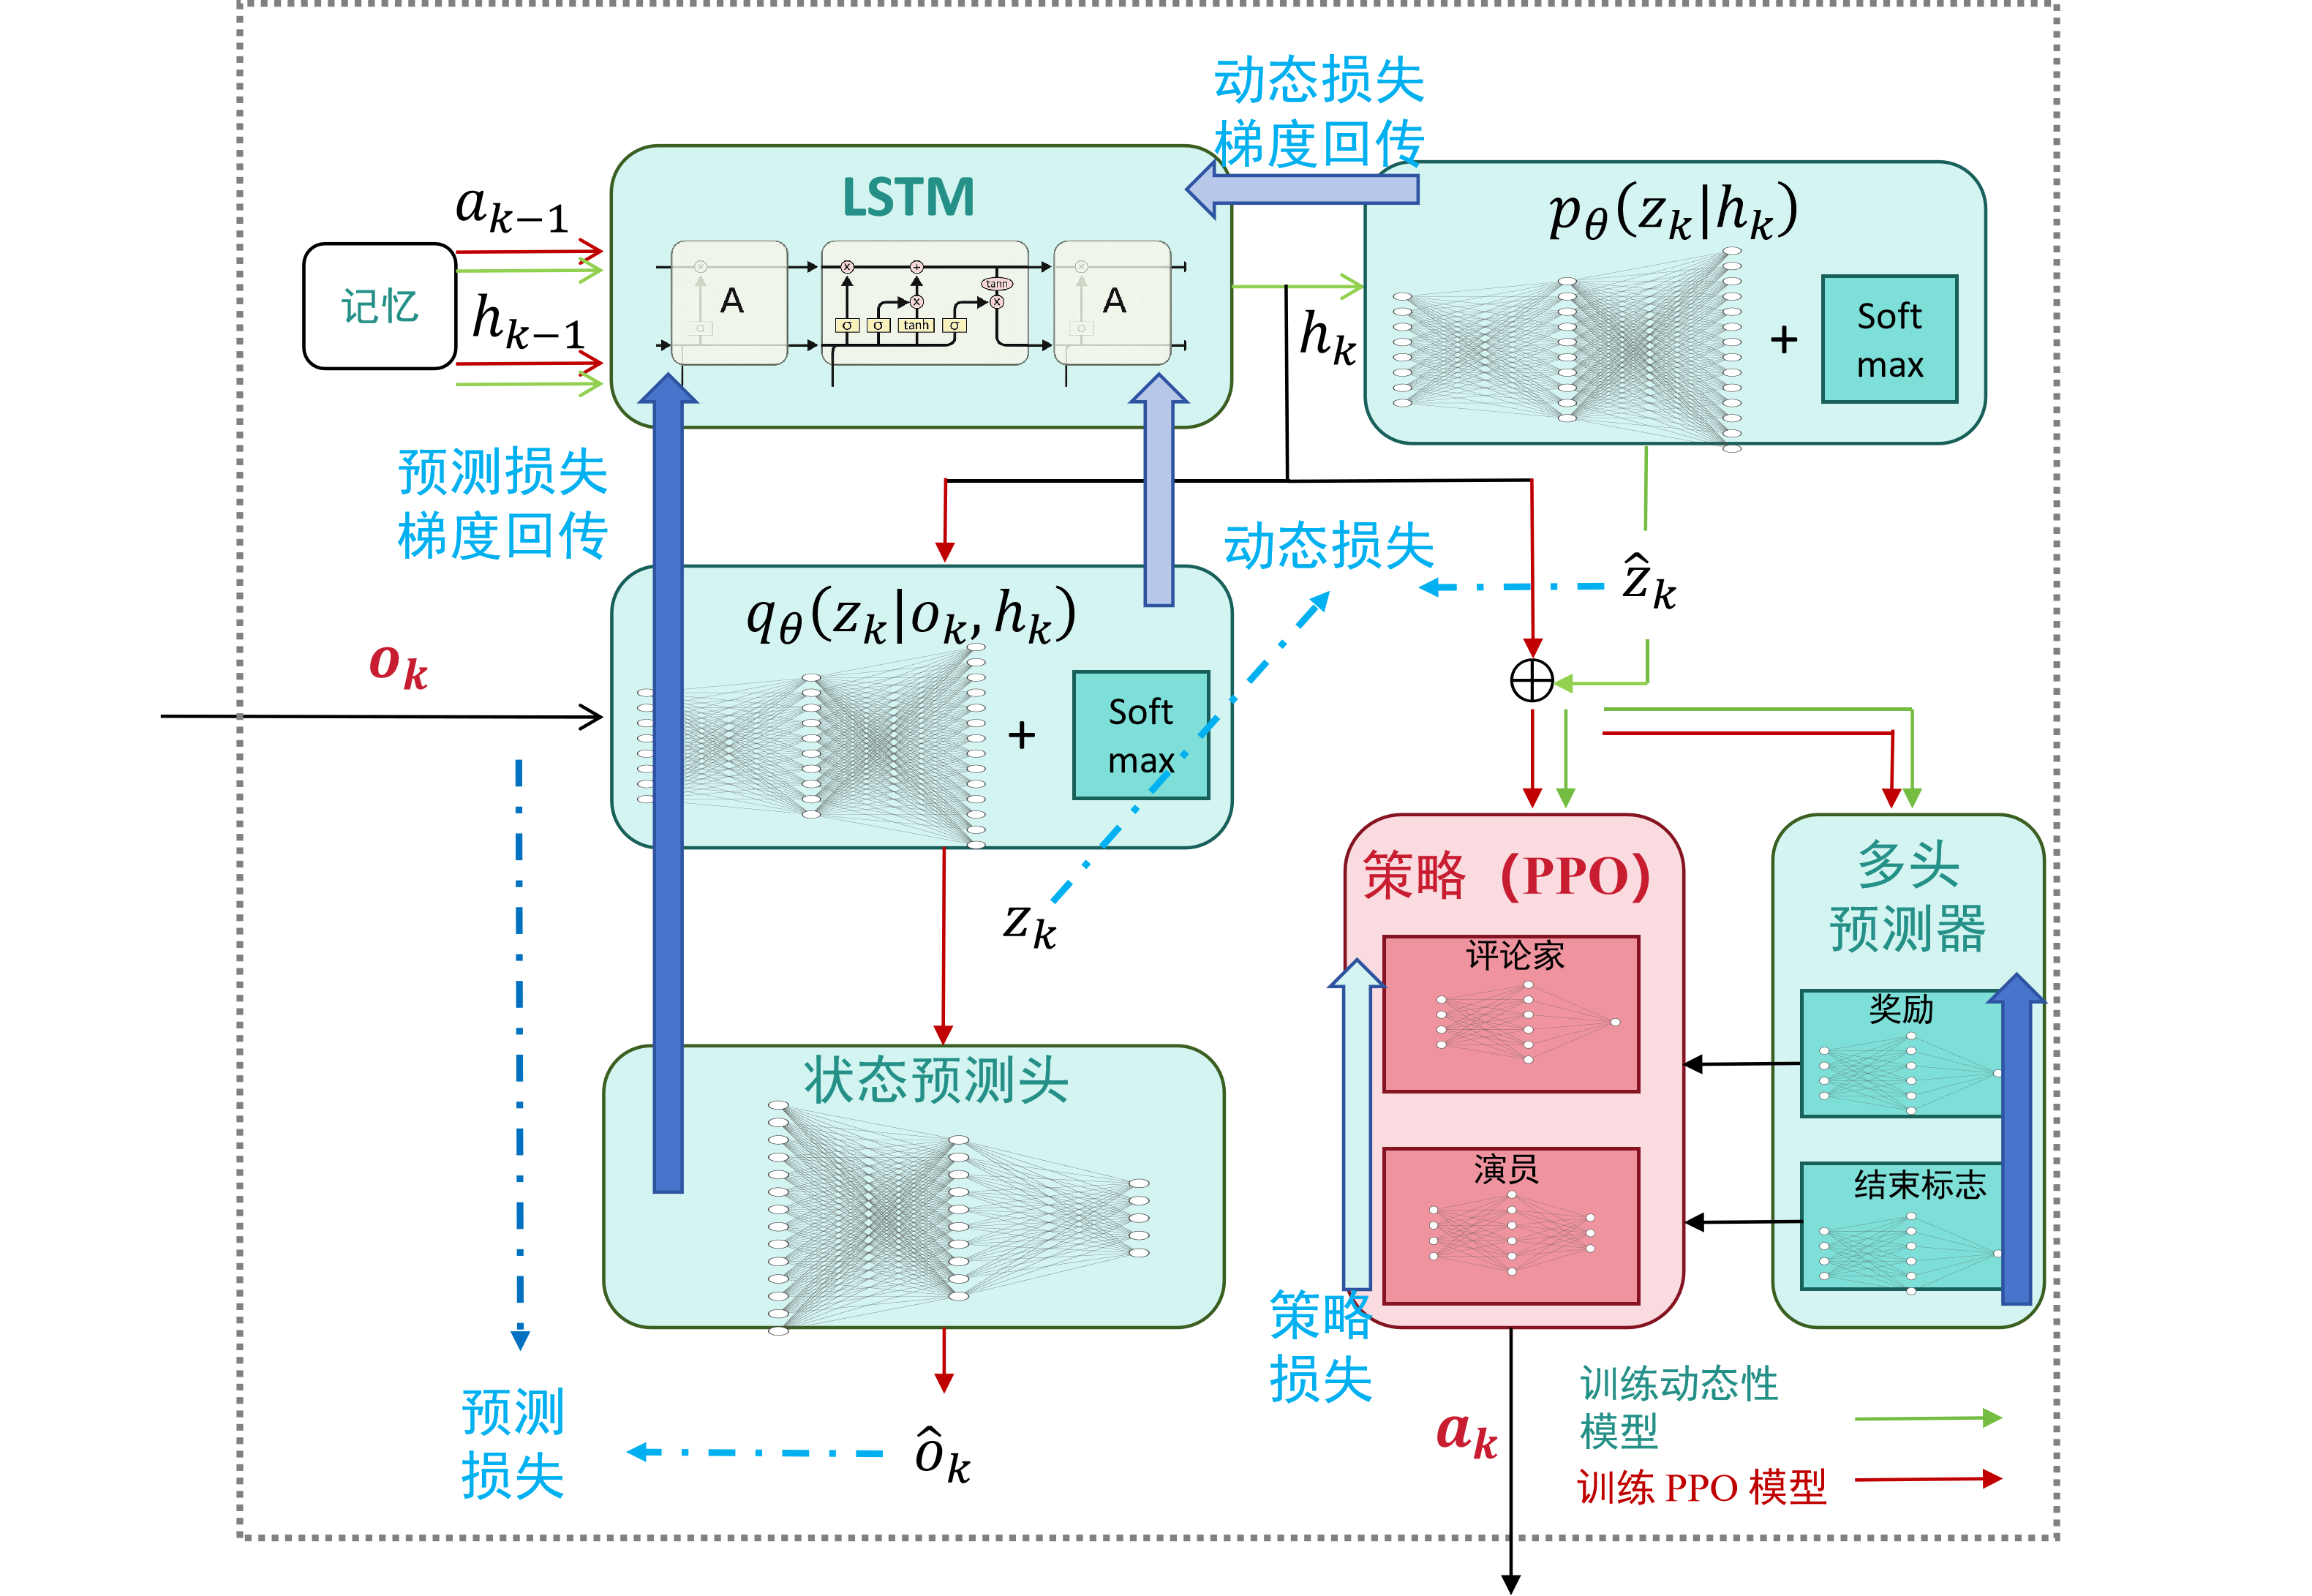
\includegraphics[width=0.9\linewidth]{figures/chapter4/Fig4_wmArchitecture.png}
    \caption{基于世界模型的生成式切片资源预留模块的神经网络结构与训练损失传播}
    \label{fig:ch4_wm_arch}
\end{figure}

\textbf{想象前向推演与策略优化.} 训练后的世界模型无需与真实 LEO-sRAN 环境交互即可生成想象切片轨迹。从当前活跃记忆状态出发，模型由先验网络采样后续隐状态并递归展开未来切片状况，所得想象轨迹为 $\mathbf{P2}$ 的奖励与可行性代理提供预测的切片满足、预留代价与 QoS 违背率。在一段想象的资源预算序列下，隐状态递归传播为
\begin{equation}\label{eq:ch4_imagine}
\boldsymbol h_{k+\tau+1}=f_\theta\!\left(\boldsymbol h_{k+\tau},\boldsymbol z_{k+\tau},\mathbf a_s(k+\tau)\right),\qquad
\boldsymbol z_{k+\tau+1}\sim p_\theta\!\left(\boldsymbol z_{k+\tau+1}\mid\boldsymbol h_{k+\tau+1}\right).
\end{equation}
累积想象奖励估计当前及未来切片动作的长期效应，用于训练切片策略而非在线求解显式的多步优化问题；想象阶段因缺乏未来物理观测，后验网络不参与。在此基础上，将学习到的世界模型与 PPO 集成~\cite{Li-EnergyBalancingOffloading-TGCN26}：确定性记忆状态 $\boldsymbol h_k$ 聚合历史状态与资源决策，先验与后验模块支配隐空间跟踪；通过对齐先验与后验，模型习得可在无需未来真实观测的条件下评估未来切片级 QoS 可行性的隐表征，用于策略训练。图~\ref{fig:ch4_wm_workflow}~在时间轴上展示了世界模型每个切片间隔的推理步骤：记忆更新、后验隐状态推断、预测头输出、先验前向推演与在线后验校正。

\begin{figure}[!htp]
    \centering
    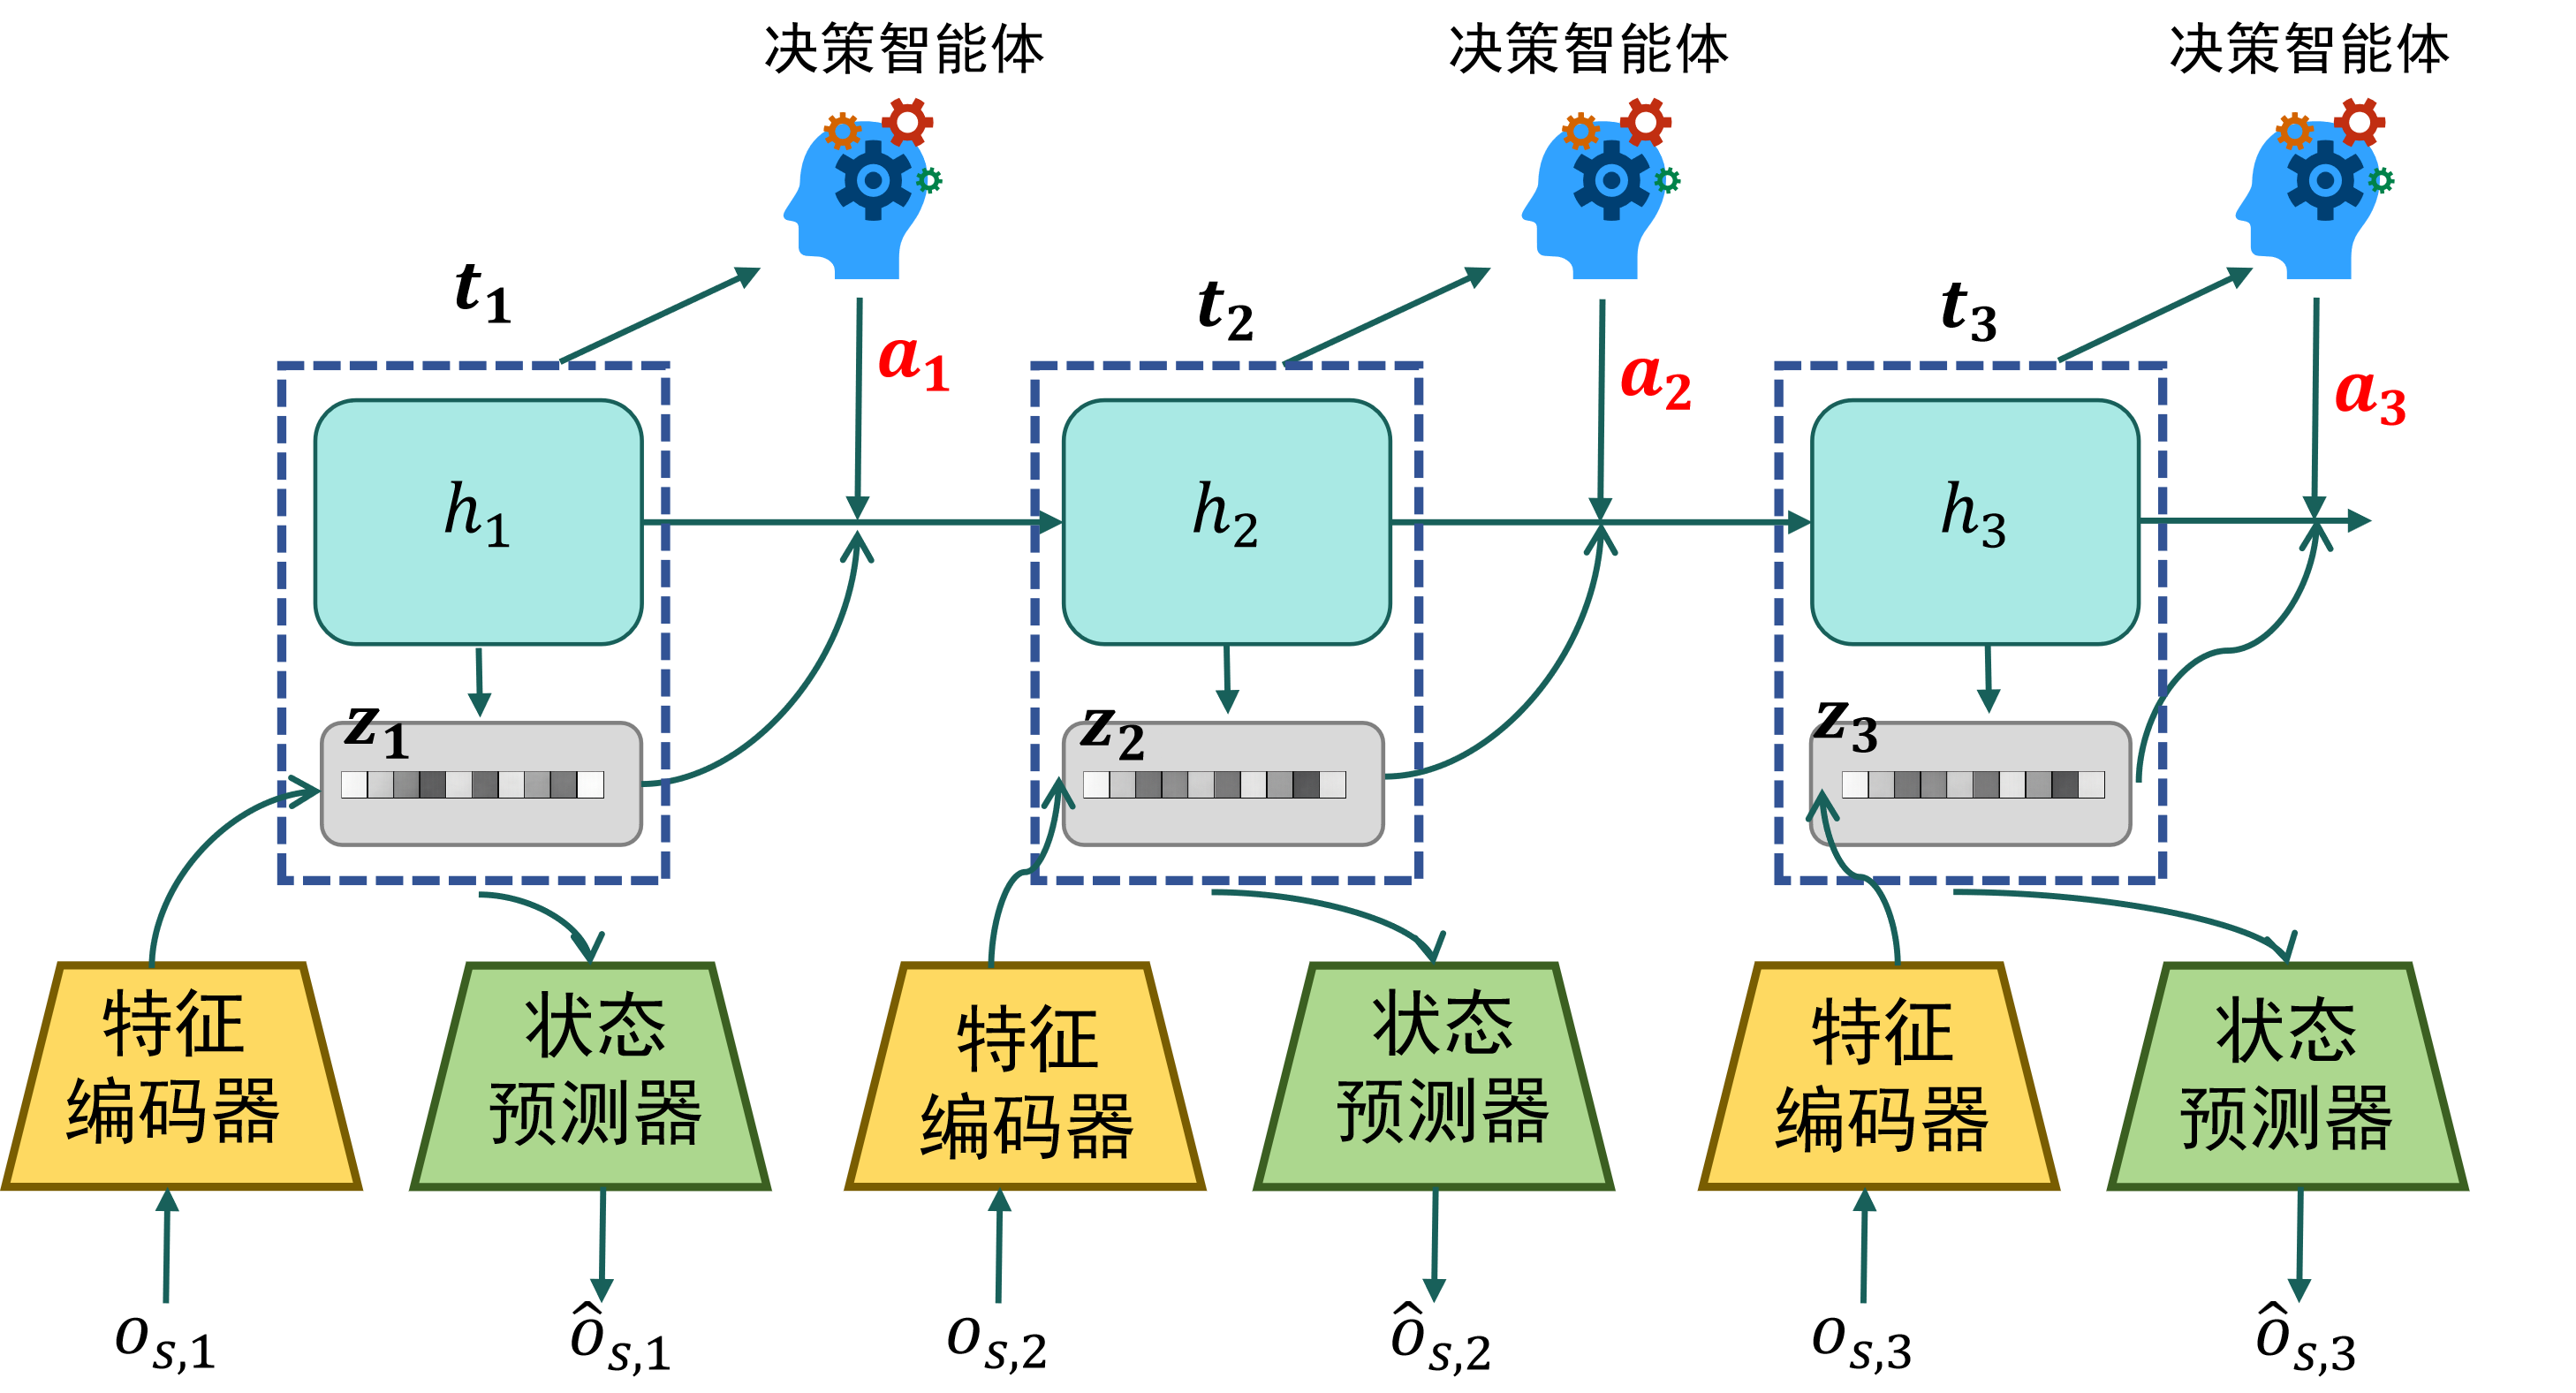
\includegraphics[width=0.92\linewidth]{figures/chapter4/Fig5_wmWorkflow.png}
    \caption{世界模型在时间轴上的逐间隔推理流程}
    \label{fig:ch4_wm_workflow}
\end{figure}

世界模型与基于 PPO 的切片策略交替训练。世界模型训练阶段，以真实轨迹推断后验隐状态、重构观测并预测预留代价与 QoS 违背率，由预测损失与先验—后验对齐损失更新记忆模块、先验网络、后验网络与预测头。策略训练阶段，冻结世界模型并将其用作想象模拟器：从当前隐状态出发，先验网络在切片策略所产生动作下递归生成想象的未来隐状态，并据此导出预留代价、QoS 违背率与想象奖励，PPO 随后以想象轨迹更新策略与评论家网络。每次策略更新时，想象前向推演由近期采集轨迹批中采样的后验隐状态初始化，而非仅从最新轨迹的终止状态出发，以改善切片状态覆盖并稳定长视野策略学习。算法~\ref{algo:ch4_slicing} 给出该交替优化流程。

\begin{algorithm}[!htp]
\caption{基于世界模型的生成式切片资源预留训练}
\label{algo:ch4_slicing}
\KwIn{环境 $\mathcal E$，预测视野 $H_p$，迭代次数 $N_{\mathrm{iter}}$}
\KwOut{训练后的世界模型与切片策略}
初始化 LSTM 记忆模块 $f_{\theta_f}$、先验网络 $p_{\theta_p}$、后验网络 $q_{\theta_q}$、观测预测头 $g_{\theta_o}$、预留代价预测头 $g_{\theta_C}$、QoS 违背率预测头 $g_{\theta_\rho}$、切片满足预测头 $g_{\theta_S}$、切片策略 $\pi_\psi$ 与评论家网络 $V_\omega$，记世界模型参数 $\Theta_{\mathrm{wm}}=\{\theta_f,\theta_p,\theta_q,\theta_o,\theta_C,\theta_\rho,\theta_S\}$\;
\For{$n\leftarrow 1$ \KwTo $N_{\mathrm{iter}}$}{
  从 $\mathcal E$ 采集轨迹 $\mathcal D^{(n)}=\{(o_{s,k},\mathbf a_s(k),C_s(k),\rho_s(k))\}_{k=1}^{T}$\;
  \For{$k\leftarrow 1$ \KwTo $T$}{
    \tcc{更新记忆与隐状态}
    $\boldsymbol h_k=f_{\theta_f}(\boldsymbol h_{k-1},\boldsymbol z_{k-1},\mathbf a_s(k-1))$\;
    $\boldsymbol z_k=q_{\theta_q}(\boldsymbol h_k,o_{s,k})$\;
    计算先验分布 $p_{\theta_p}(\boldsymbol z_k\mid\boldsymbol h_k)$，用于式~\eqref{eq:ch4_ldyn} 的先验—后验对齐\;
    \tcc{重构观测并预测性能指标}
    $\hat o_{s,k}=g_{\theta_o}(\boldsymbol h_k,\boldsymbol z_k)$，$\hat C_s(k)=g_{\theta_C}(\boldsymbol h_k,\boldsymbol z_k)$，$\hat\rho_s(k)=g_{\theta_\rho}(\boldsymbol h_k,\boldsymbol z_k)$，$\hat S_{s,c}^{\mathrm{slice}}(k)=g_{\theta_S}(\boldsymbol h_k,\boldsymbol z_k),\forall c\in\mathcal C$\;
  }
  \tcc{优化世界模型参数}
  $\Theta_{\mathrm{wm}}\leftarrow\Theta_{\mathrm{wm}}-\alpha_d\nabla_{\Theta_{\mathrm{wm}}}\mathcal L_{\mathrm{wm}}$\;
  冻结 $\Theta_{\mathrm{wm}}$，由 $\mathcal D^{(n)}$ 中隐状态初始化想象前向推演\;
  \For{$\tau\leftarrow 0$ \KwTo $H_p-1$}{
    \tcc{经冻结世界模型生成想象转移}
    $\mathbf a_s(k+\tau)=\pi_\psi(\boldsymbol h_{k+\tau},\boldsymbol z_{k+\tau})$\;
    $\boldsymbol h_{k+\tau+1}=f_{\theta_f}(\boldsymbol h_{k+\tau},\boldsymbol z_{k+\tau},\mathbf a_s(k+\tau))$\;
    $\boldsymbol z_{k+\tau+1}\sim p_{\theta_p}(\cdot\mid\boldsymbol h_{k+\tau+1})$\;
    $\hat C_s(k+\tau)=g_{\theta_C}(\cdot)$，$\hat\rho_s(k+\tau)=g_{\theta_\rho}(\cdot)$，$\hat S_{s,c}^{\mathrm{slice}}(k+\tau)=g_{\theta_S}(\cdot),\forall c\in\mathcal C$\;
    按罚项奖励构造 $\hat R_s(k+\tau)$\;
  }
  \tcc{构造想象轨迹并更新 PPO}
  构造 $\hat{\mathcal D}^{(n)}=\{(\boldsymbol h_{k+\tau},\boldsymbol z_{k+\tau},\mathbf a_s(k+\tau),\hat R_s(k+\tau))\}_{\tau=0}^{H_p-1}$\;
  $\Theta_\pi=\{\psi,\omega\}$，$\Theta_\pi\leftarrow\Theta_\pi+\alpha_\pi\nabla_{\Theta_\pi}\mathcal L_{\mathrm{PPO}}(\hat{\mathcal D}^{(n)})$\;
}
\end{algorithm}

生成式切片资源预留模块的输出为切片级资源包络 $\{W_{s,c}(k),P_{s,c}(k)\}_{c\in\mathcal C}$ 与本地关联调整 $\mathbf m_s(k)$。这些决策既不包含预测的 MAC 层调度变量，也不指定时隙级 RBG 指派或流级功率分配，而是界定 MAC 调度器执行 QoS 可行性感知的业务流选择与资源映射的可行域，相应的快时间尺度调度机制见第~\ref{subsec:ch4_mac}~节。

\subsection{QCI 优先级背包 MAC 调度}
\label{subsec:ch4_mac}

生成式切片资源预留在切片层面提升了异构 QoS 保障的长期可行性。快时间尺度问题则是切片级带宽与功率预算下针对各业务流的 MAC 调度：在给定预算内，MAC 调度器须确定当前时隙服务哪些业务流，并确保被选中流以所消耗资源满足其 QoS 需求。以李雅普诺夫方法为代表的队列型调度器经积压或亏损压力间接调节 QoS，但高队列权重并不意味着用户的 QoS 需求在当前信道与切片预算下可满足。服务此类用户可能耗费稀缺的 RBG 或功率，却仍无法满足其 QoS 门限。因此，本节不再最大化队列加权吞吐或额外求解连续功率分配问题，而是将 MAC 层调度形式化为 QoS 可行性感知的资源选择问题。

\textbf{最小 RBG—功率需求估计.} 调度器在资源选择前，先将每条业务流的 QoS 需求转化为最小 RBG—功率需求。这一映射在 LEO-sRAN 中可解析处理，因为下行信道由大尺度传播损耗主导：给定卫星星历与终端位置，星地距离可在一个较短的 MAC 时隙内预测，相应信道增益 $h_{i,s}(t)$ 可由大尺度路径损耗模型估计。记卫星 $s$ 在时隙 $t$ 为业务流 $i$ 分配 $n_i(t)$ 个 RBG，对应带宽为 $B_i(n_i)=n_iB_g$，则在 RBG 数 $n_i(t)$ 与发射功率 $p_i(t)$ 下，流 $i$ 的传输速率为
\begin{equation}\label{eq:ch4_apprate}
r_i(n_i,p_i;t)=n_iB_g\log_2\!\left(1+\frac{p_i(t)G_sG_uh_{i,s}(t)}{N_0n_iB_g}\right).
\end{equation}
由于式~\eqref{eq:ch4_rateutil}--\eqref{eq:ch4_delayutil} 的 QoS 效用同时依赖传输速率与时延，先推导流 $i$ 满足其 QoS 门限所需的最小服务速率，定义为
\begin{equation}\label{eq:ch4_reqrate}
r_i^{\mathrm{req}}(t)=\inf\left\{r>0:\xi_{c_i}S_i^{\mathrm{rate}}(r)+(1-\xi_{c_i})S_i^{\mathrm{delay}}\!\left(d_i(r;t)\right)\ge S_i^{\min}\right\},
\end{equation}
其中 $d_i(r;t)$ 按第~\ref{subsec:ch4_link}~节的时延模型评估。对候选服务速率 $r$，时延近似为
\begin{equation}\label{eq:ch4_delaygivenrate}
d_i(r;t)=\frac{\ell}{r}+d_i^{\mathrm{prop}}(t)+\frac{\lambda_{m_i}}{(r/\ell)\big(r/\ell-\lambda_{m_i}\big)}.
\end{equation}
若 $r/\ell\le\lambda_{m_i}$，则 M/M/1 时延近似失效，该候选服务速率被判为不可行。对给定 RBG 数 $n_i$，达到 $r_i^{\mathrm{req}}(t)$ 所需的最小发射功率可由反演式~\eqref{eq:ch4_apprate} 得到，即
\begin{equation}\label{eq:ch4_minpower}
p_i^{\min}(n_i,t)=\frac{N_0n_iB_g}{G_sG_uh_{i,s}(t)}\left(2^{\frac{r_i^{\mathrm{req}}(t)}{n_iB_g}}-1\right).
\end{equation}
该式给出流 $i$ 在每个候选 RBG 指派下的显式功率开销。对相同所需速率，分配更多 RBG 可降低所需发射功率，分配更少 RBG 则节省带宽但可能耗费过量功率。由于后续背包问题同时受 RBG 与功率预算约束，每条候选流须以单一可执行的 RBG—功率对表示。记切片 $c$ 的 RBG 预算为 $N_{s,c}^{\mathrm{RBG}}(k)=\lfloor W_{s,c}(k)/B_g\rfloor$。为在同一尺度上比较异构的带宽与功率开销，将每个资源维以相应切片预算归一化，并选取消耗切片资源组合占比最小的资源对：
\begin{equation}\label{eq:ch4_minpair}
(n_i^{\min}(t),p_i^{\min}(t))=\arg\min_{1\le n_i\le N_{s,c}^{\mathrm{RBG}}(k)}\left(\frac{n_i}{N_{s,c}^{\mathrm{RBG}}(k)}+\frac{p_i^{\min}(n_i,t)}{P_{s,c}(k)}\right),
\end{equation}
约束为 $p_i^{\min}(n_i,t)\le P_{s,c}(k)$。若不存在满足 $p_i^{\min}(n_i,t)\le P_{s,c}(k)$ 的 $n_i$，则流 $i$ 在当前时隙不可行，被排除出候选物品集；该条件滤除在当前切片预算与链路条件下无法被单独支撑的业务流，而被选流之间聚合的 RBG 与功率可行性由后续背包约束保证。

\textbf{背包物品构造.} 完成最小资源需求估计后，每条可行业务流被建模为一个背包物品：物品价值由 QCI/5QI 导出的优先级值定义，物品权重对应所需 RBG 数与发射功率。记流 $i$ 的标准化 QCI/5QI 标识为 $q_i$。由于 QCI/5QI 标识规定的是标准化 QoS 类别而非序数化的数值优先级，不直接将其用作物品价值，而是依据 $q_i$ 关联的标准化 QoS 特征（如优先级等级、分组时延预算与业务类别）为每条流赋予 QCI 导出优先级值 $\pi_i$，并令物品价值 $v_i=\pi_i$。该选择保留了标准化的业务等级区分，同优先级流的取舍由其所需 RBG—功率开销决定；紧迫度感知的物品赋值留作后续工作。

\textbf{二维背包与动态规划求解.} 记切片 $c$ 在卫星 $s$ 时隙 $t$ 的可行流集合为 $\mathcal I_{s,c}^{\mathrm{fea}}(t)$。MAC 调度问题随即近似为二维 0--1 背包问题：
\begin{equation}\label{eq:ch4_knapsack}
\begin{aligned}
\max_{\{y_i(t)\}}\ &\sum_{i\in\mathcal I_{s,c}^{\mathrm{fea}}(t)}\pi_iy_i(t)\\
\text{s.t.}\ &\sum_{i\in\mathcal I_{s,c}^{\mathrm{fea}}(t)}n_i^{\min}(t)y_i(t)\le N_{s,c}^{\mathrm{RBG}}(k),\\
&\sum_{i\in\mathcal I_{s,c}^{\mathrm{fea}}(t)}p_i^{\min}(t)y_i(t)\le P_{s,c}(k),\\
&y_i(t)\in\{0,1\},\quad\forall i\in\mathcal I_{s,c}^{\mathrm{fea}}(t).
\end{aligned}
\end{equation}
二值变量 $y_i(t)$ 指示业务流 $i$ 是否在时隙 $t$ 被选中。由于每个可行物品在 $(n_i^{\min}(t),p_i^{\min}(t))$ 下均满足 $S_i(t)\ge S_i^{\min}$，选中物品 $i$ 等价于服务一条满足 $\mathbf{P3}$ 中 QoS 约束的业务流；因此式~\eqref{eq:ch4_knapsack} 在以可执行的最小资源开销替代连续带宽—功率决策变量的同时，保留了 $\mathbf{P3}$ 优先级加权的满足目标。式~\eqref{eq:ch4_knapsack} 的二维背包问题在将功率预算量化为离散单元后经动态规划求解。记功率粒度为 $\Delta P$，量化功率开销为 $\bar p_i^{\min}(t)=\lceil p_i^{\min}(t)/\Delta P\rceil$，功率容量为 $\bar P_{s,c}(k)=\lfloor P_{s,c}(k)/\Delta P\rfloor$。定义 $F_i(n,p)$ 为在前 $i$ 个可行流、至多 $n$ 个 RBG 与 $p$ 个功率单元下可获得的最大 QCI 优先级值，其递推为
\begin{equation}\label{eq:ch4_dp}
F_i(n,p)=\max\left\{F_{i-1}(n,p),\,F_{i-1}\!\left(n-n_i^{\min},p-\bar p_i^{\min}\right)+\pi_i\right\},
\end{equation}
当 $n\ge n_i^{\min}$ 且 $p\ge\bar p_i^{\min}$ 时成立，否则 $F_i(n,p)=F_{i-1}(n,p)$。回溯动态规划表即可确定当前时隙被选中的业务流集合。

\textbf{资源执行.} 选定业务流后，直接执行如下资源分配规则。由于信道模型由大尺度路径损耗主导，给定业务流在当前时隙内所有 RBG 经历相同的链路条件，调度器将每条被选流映射至切片内任意可用的 $n_i^{\min}(t)$ 个 RBG，并对所有 $y_i(t)=1$ 的被选流置 $B_i(t)=n_i^{\min}(t)B_g$、$p_{i,s}(t)=p_i^{\min}(t)$；对未选中流不分配带宽与功率。该执行规则使背包选择所用的资源开销估计与实际 MAC 层分配保持一致，并避免额外的凸功率优化阶段。算法~\ref{algo:ch4_knapsack} 总结了 QCI 优先级背包 MAC 调度流程。

\begin{algorithm}[!htp]
\caption{QCI 优先级背包 MAC 调度}
\label{algo:ch4_knapsack}
\KwIn{切片级带宽预算 $\{W_{s,c}(k)\}_{c\in\mathcal C}$、切片级功率预算 $\{P_{s,c}(k)\}_{c\in\mathcal C}$、候选流集合 $\{\mathcal I_{s,c}(k)\}_{c\in\mathcal C}$、QCI/5QI 标识 $\{q_i\}$、QCI 导出优先级值 $\{\pi_i\}$、大尺度信道增益 $\{h_{i,s}(t)\}$}
\KwOut{RBG 指派 $\mathbf X_s(t)$ 与功率分配 $\mathbf p_s(t)$}
\For{每类切片 $c\in\mathcal C$}{
  $N_{s,c}^{\mathrm{RBG}}(k)=\lfloor W_{s,c}(k)/B_g\rfloor$\;
  初始化可行物品集 $\mathcal I_{s,c}^{\mathrm{fea}}(t)=\emptyset$\;
  \tcc{构造 QoS 可行背包物品}
  \For{每条流 $i\in\mathcal I_{s,c}(k)$}{
    按式~\eqref{eq:ch4_reqrate} 计算 $r_i^{\mathrm{req}}(t)$\;
    \For{$n_i\leftarrow 1$ \KwTo $N_{s,c}^{\mathrm{RBG}}(k)$}{
      按式~\eqref{eq:ch4_minpower} 计算 $p_i^{\min}(n_i,t)$\;
    }
    按式~\eqref{eq:ch4_minpair} 求 $(n_i^{\min}(t),p_i^{\min}(t))$\;
    \If{存在可行资源对}{
      将流 $i$ 以价值 $\pi_i$、权重 $(n_i^{\min}(t),p_i^{\min}(t))$ 加入 $\mathcal I_{s,c}^{\mathrm{fea}}(t)$\;
    }
  }
  \tcc{经动态规划求解二维 0--1 背包}
  以 $\Delta P$ 量化功率开销并构造动态规划表 $F_i(n,p)$\;
  按式~\eqref{eq:ch4_dp} 更新 $F_i(n,p)$\;
  回溯动态规划表得被选流 $\{i:y_i(t)=1\}$\;
  \tcc{执行所选资源分配}
  \For{每条被选流 $i$}{
    将流 $i$ 映射至切片 $c$ 内任意可用的 $n_i^{\min}(t)$ 个 RBG\;
    置 $B_i(t)=n_i^{\min}(t)B_g$、$p_{i,s}(t)=p_i^{\min}(t)$\;
  }
  \For{每条未选中流 $i$}{
    置 $B_i(t)=0$、$p_{i,s}(t)=0$\;
  }
}
\end{algorithm}

\subsection{框架工作流与复杂度分析}
\label{subsec:ch4_workflow}

\textbf{整体工作流.} DTPS 的端到端工作流如图~\ref{fig:ch4_dtps_workflow}~所示。在每个切片间隔起始，切片层更新记忆状态、由当前观测推断后验隐状态，并确定切片级带宽与功率预算以及本地关联调整，这些决策参数化随后 MAC 执行的可行域。在每个 MAC 时隙内，调度器在当前大尺度信道状态下评估候选业务流的 QoS 可行资源需求，经 QCI 优先级背包选取优先级加权的可行子集，并直接执行相应的 RBG—功率分配。实现的服务统计随后反馈至切片层，触发后验校正与后续的预测式预算，由此形成慢/快两个时间尺度上的闭环。

\begin{figure}[!htp]
    \centering
    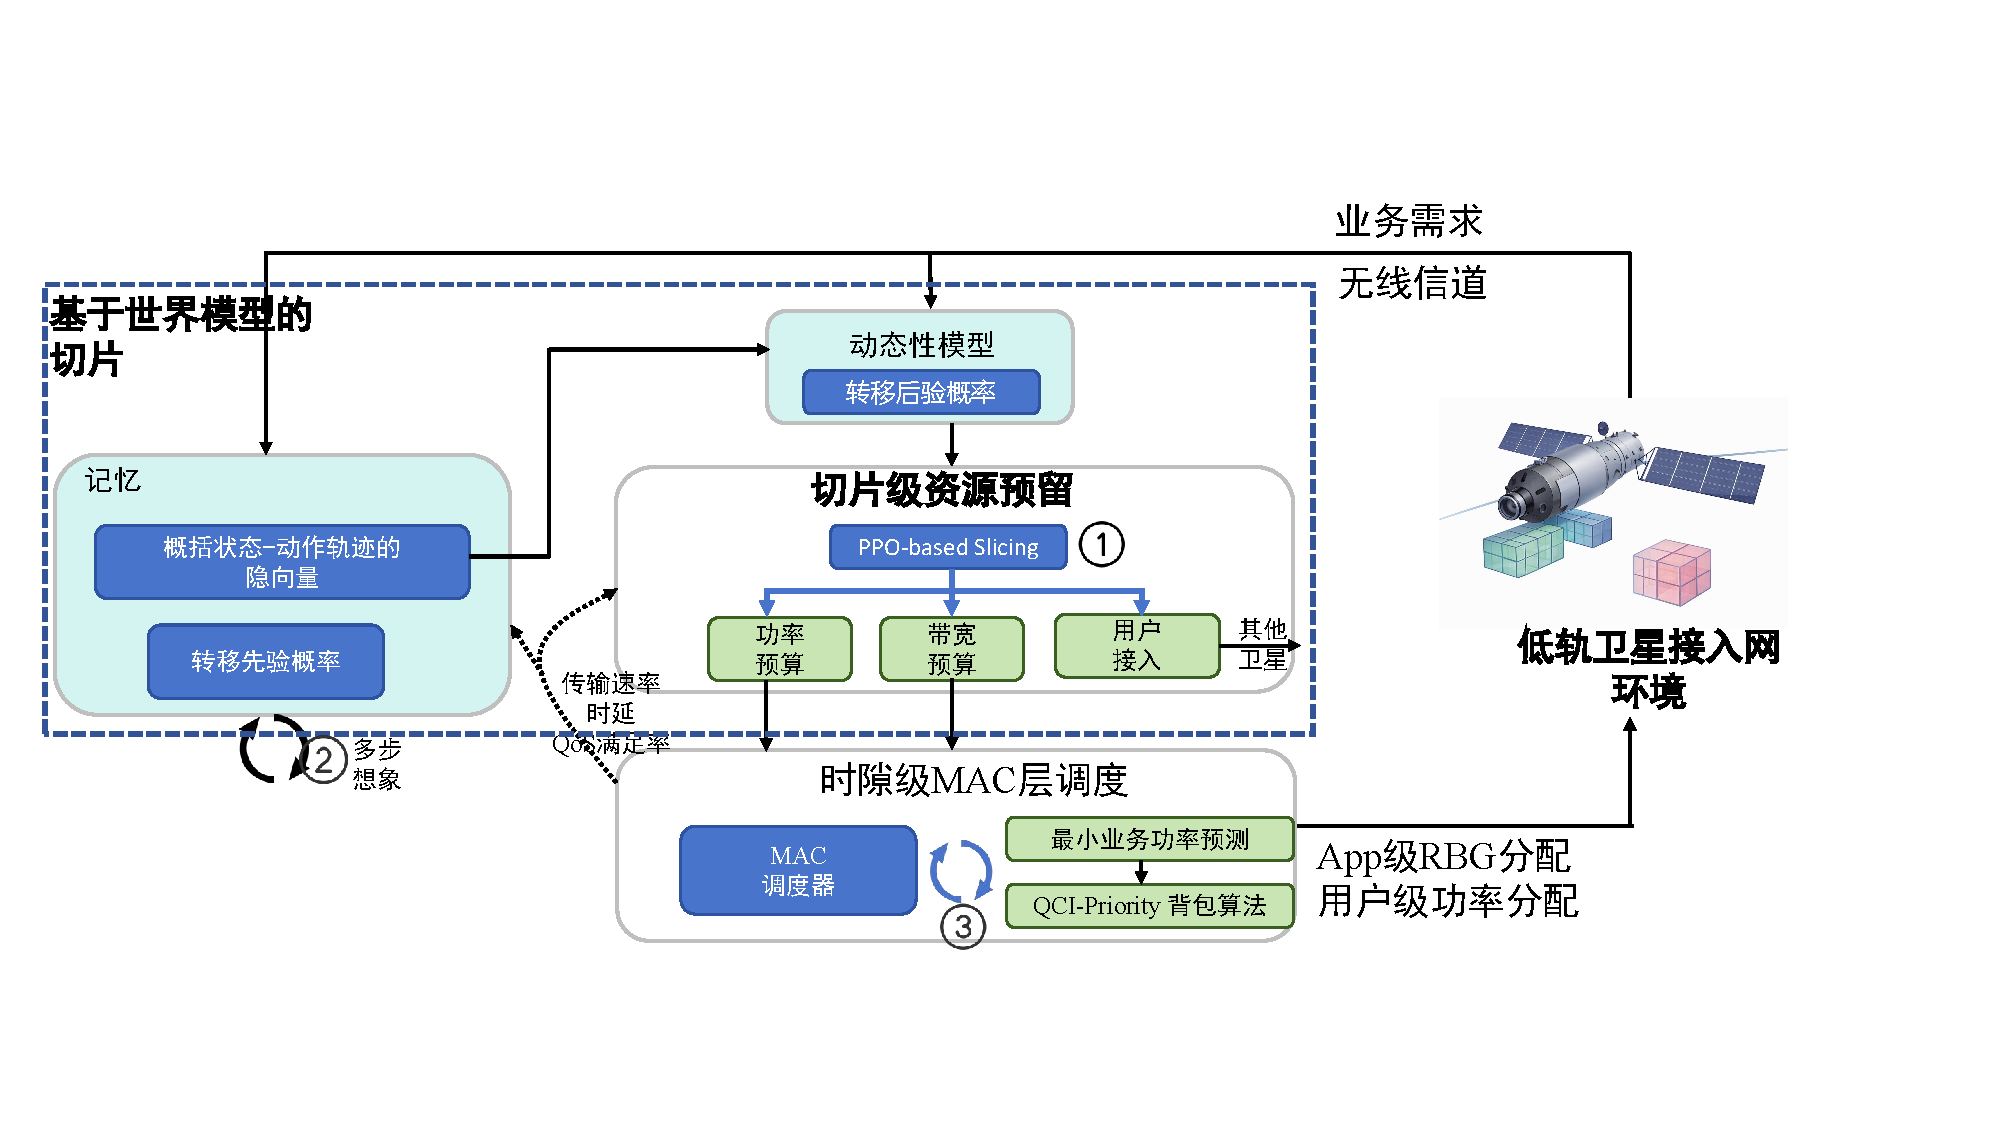
\includegraphics[width=0.86\linewidth]{figures/chapter4/Figure6_workflow.pdf}
    \caption{DTPS 框架的整体工作流}
    \label{fig:ch4_dtps_workflow}
\end{figure}

\textbf{复杂度分析.} DTPS 的复杂度由慢时间尺度的生成式切片资源预留与快时间尺度的 MAC 调度两部分构成。在切片层，世界模型推断与 PPO 策略评估在每个切片间隔仅基于聚合的切片级与业务类型描述符执行一次，因而其复杂度与业务流数无关，可记为 $\mathcal O(C_{\mathrm{wm}}+C_\pi)$，其中 $C_{\mathrm{wm}}$ 与 $C_\pi$ 分别为潜动态模型与切片策略的固定推断开销。在 MAC 层，对卫星 $s$ 上的切片 $c$，记候选流数与可行流数分别为 $A_{s,c}=|\mathcal I_{s,c}(k)|$ 与 $A_{s,c}^{\mathrm{fea}}=|\mathcal I_{s,c}^{\mathrm{fea}}(t)|$。最小资源估计的复杂度为 $\mathcal O(A_{s,c}N_{s,c}^{\mathrm{RBG}})$，二维动态规划背包的复杂度为 $\mathcal O(A_{s,c}^{\mathrm{fea}}N_{s,c}^{\mathrm{RBG}}\bar P_{s,c})$，故每时隙 MAC 复杂度为
\begin{equation}\label{eq:ch4_complexity}
\mathcal O\!\left(\sum_{c\in\mathcal C}\big(A_{s,c}N_{s,c}^{\mathrm{RBG}}+A_{s,c}^{\mathrm{fea}}N_{s,c}^{\mathrm{RBG}}\bar P_{s,c}\big)\right).
\end{equation}
尽管动态规划步骤为伪多项式，但 $N_{s,c}^{\mathrm{RBG}}$ 与 $\bar P_{s,c}$ 受切片级预算与功率量化粒度限定，且不可行流在动态规划前已被滤除。因此，DTPS 使慢时间尺度推断与活跃业务流数无关，并将快时间尺度调度限定在受预算界定的离散搜索空间内，适合星上的快时间尺度执行。

\section{仿真实验与性能分析}
\label{sec:ch4_experiments}

本节通过大规模仿真评估所提 DTPS 框架，重点考察四个方面：不同业务负载下的整体 QoS 保障、由业务突发引起的服务不确定性下的鲁棒性、基于世界模型的生成式切片资源预留机制的贡献，以及固定切片预算下 QoS 可行性感知 MAC 调度器的独立效果。评估以 QoS 满足率为主要指标，并以加权资源消耗为资源效率指标。

\subsection{仿真设置}
\label{subsec:ch4_setup}

大规模 LEO 星座按 Starlink Phase~1 Shell~1 单层架构建模~\cite{Bhattacherjee-NetworkTopology-Conext19}，含 72 个轨道面、每面 22 颗卫星。为在时变服务条件下评估长期资源预留，仿真以回合（episode）组织：每个回合时长 $200$~s，对应 400 个切片间隔，并对应第~\ref{subsec:ch4_network}~节中可见关系保持不变的一个调度区间；共运行 5 个回合，合计 2000 个切片间隔、总时长 $1000$~s。每个切片间隔取 $0.5$~s，以兼顾星上计算约束、AI 模型推断时延与 LEO 信令开销~\cite{yao-LEOEdge-JSAC25}；每个切片周期内 MAC 调度器运行 50 个时隙，每时隙时长 $10$~ms，与标准 4G LTE 无线帧对齐~\cite{3gpp_ts_36_211}。目标仿真区域为美国东海岸附近的矩形区域~\cite{liu-reconfigurableRanSlicing-TCCN25}，纬度 $31.5^\circ$N 至 $33^\circ$N、经度 $79.5^\circ$W 至 $81^\circ$W，在 $40^\circ$ 最小仰角约束下选取在每个回合内对目标区域可见关系保持不变的卫星集合，回合之间按星历更新可见卫星集合。在缺乏公开 LEO 业务轨迹的情况下，依据 3GPP 5G 系统架构的业务类别生成合成业务负载~\cite{etsi_3gpp_5g_system_architecture_2018}，考虑视频会议、视频流、车联网（Vehicle-to-Everything，V2X）与虚拟现实（Virtual Reality，VR）卸载四类业务。切片归属由各业务的主导 QoS 需求而非 QCI/5QI 标识决定：速率需求较高的业务归入带宽密集型切片，时延需求严格的业务归入时延敏感型切片，因而视频会议与视频流归为带宽密集型，V2X 与 VR 卸载归为时延敏感型；表~\ref{tab:ch4_traffic} 中的 QCI/5QI 标识仅用于导出 MAC 层业务优先级值 $\pi_i$。

\begin{table}[!htp]
\centering
\caption{主要仿真参数}
\label{tab:ch4_params}
\small
\renewcommand{\arraystretch}{1.2}
\begin{tabular}{lclc}
\toprule
参数 & 取值 & 参数 & 取值 \\
\midrule
$W_s$ & $20$~MHz & $P_s^{\max}$ & $40$~dBm \\
$f_c$ & $4$~GHz & $N_0$ & $-174$~dBm/Hz \\
$G_sG_u$ & $30$~dBi & RBG 数 & $27$ \\
$\ell$ & $250$~Bytes & $(\eta_W,\eta_P)$ & $(2.0,0.5)$ \\
\bottomrule
\end{tabular}
\end{table}

\begin{table}[!htp]
\centering
\caption{实验选取的业务类型}
\label{tab:ch4_traffic}
\small
\renewcommand{\arraystretch}{1.2}
\begin{tabular}{lccc}
\toprule
业务类型 & 最小吞吐 & 最大时延 & QCI/5QI \\
\midrule
视频会议 & $2$~Mbps & $150$~ms & $40$ \\
视频流 & $2$~Mbps & $300$~ms & $60$ \\
V2X & $200$~kbps & $50$~ms & $40$ \\
VR 卸载 & $10$~Mbps & $30$~ms & $68$ \\
\bottomrule
\end{tabular}
\end{table}

业务与负载设置服务于第~\ref{subsec:ch4_exp_load}~节不同负载下的 QoS 保障评估。基于 GeoLite2~\cite{maxmind_geolite2_2021} 的 IP--位置数据库，在目标区域内识别出 46 个潜在用户并假定其在区域内均匀分布；初始时每个用户按第~\ref{subsec:ch4_network}~节的规则接入可见范围内距离最近的卫星，运行期间的关联调整方式见下文方法设置。为刻画异构业务需求，允许每个物理用户产生至多两条逻辑应用流，每条流属于表~\ref{tab:ch4_traffic} 中四类业务之一，采样频率分别为 $45\%$、$30\%$、$15\%$ 与 $10\%$，故 46 个物理用户至多产生 92 条候选流。业务在 MAC 时隙级按式~\eqref{eq:ch4_arrival} 生成；为改变所提供的业务负载，引入激活比 $\rho$ 与到达缩放因子 $\kappa$：$\rho$ 决定 92 条候选流中活跃流的占比，$\kappa$ 缩放各活跃流的到达强度，即活跃流 $i$ 的到达率为 $\lambda_i(t)=\kappa\lambda_{m_i}$、否则为 $0$。据此在轻、中、重与过载四档负载下评估网络性能，$(\rho,\kappa)$ 分别取 $(0.40,0.8)$、$(0.55,0.9)$、$(0.70,1.0)$ 与 $(0.90,1.1)$。

服务不确定性设置服务于第~\ref{subsec:ch4_exp_burst}~节的鲁棒性评估。时隙级信道与业务波动经 On--Off 突发机制刻画：每颗卫星以概率 $p_b$ 进入突发态，低、中、高三档不确定性对应 $p_b\in\{0.005,0.015,0.05\}$；突发期内到达率与服务速率分别缩放为 $\lambda_i(t)=\nu_i(t)\kappa\lambda_{m_i}$ 与 $r_i(t)=\eta_s(t)\hat r_i(t)$，其中 $\nu_i(t)\sim\mathcal U[1,1.5]$、$\eta_s(t)\sim\mathcal U[0.7,1]$。在该多时间尺度结构下，业务到达与流级 QoS 指标在快 MAC 尺度波动，而切片级资源预算在每个切片间隔内保持不变。

其余为效用与算法参数。QoS 效用经 sigmoid 函数评估，平滑系数 $b_r=14$、$b_d=18$，满足门限 $S_i^{\min}=0.9$。式~\eqref{eq:ch4_avgcost} 与式~\eqref{eq:ch4_predcost} 中带宽消耗权重 $\eta_W$ 高于功率消耗权重 $\eta_P$（取值见表~\ref{tab:ch4_params}），以体现 QoS 受限卫星接入场景中 QoS 可行性优先于节省功率的取向：较小的功率权重允许调度器在必要时增用发射功率以满足速率—时延需求，同时仍抑制不必要的功率消耗。其余参数汇总于表~\ref{tab:ch4_params}~\cite{zhang-JointBeamformingResAlloc-SAGIN-TCOM20,wang-UserSelectionMIMO-TVT21,cybertwin-ModeSelection-LEO-IoTJ22,zhang-RISMIMO-LEO-IoTJ25,hua-GANDRL-ResourceSlicing-JSAC20}。

所提 DTPS 框架与若干代表性基线对比。TDRL-RSUA~\cite{liu-reconfigurableRanSlicing-TCCN25} 经带动作掩蔽的 PPO 优化切片级带宽与功率预算，因其不含原生 MAC 层调度器，故与文献~\cite{chai-ResAllocRANSlicing-Lyapunov-TVT25} 的时延感知李雅普诺夫资源分配方法结合以执行时隙级调度。由于用户—卫星关联不在上述基线的设计范围内，各基线在运行期间统一采用文献~\cite{Nguyen-JointAssocResAlloc-TWC24} 的负载自适应关联方案，在切片间隔间联合考虑链路质量与卫星负载更新用户—卫星关联；所提 DTPS 不依赖该外部关联方案，而是经 $\mathbf{P2}$ 中的本地关联调整 $\mathbf m_s(k)$ 在可见邻星间迁移过载业务流。RL-JRSS~\cite{wu-LearnSlicing-JCIN21} 经问题分解协调切片预留与用户调度，由 PPO 处理切片级资源分配、背包匹配执行用户调度。TDRL-RSUA 与 RL-JRSS 均增设切片级功率分配的动作头，以在多维资源控制下保持一致对比。为将世界模型与传统序列建模相比较，另实现一个 LSTM 增强基线，在基于强化学习的切片前编码历史观测。LACO~\cite{zaozi-laco-5G-TWC21} 以 QoS 违背驱动的多臂赌博机更新切片带宽份额，同样与文献~\cite{chai-ResAllocRANSlicing-Lyapunov-TVT25} 的李雅普诺夫调度器结合执行 MAC 层。DQN-MAC~\cite{AlQwider-DQN5GNR-ICC22} 作为非切片基线，以深度 Q 网络直接将用户映射至资源块、发射功率在活跃资源块上均匀分配。所有数值结果均在 10 次独立随机种子运行上平均。

\subsection{不同业务负载下的整体性能}
\label{subsec:ch4_exp_load}

首先在不同业务强度下评估整体性能。图~\ref{fig:ch4_exp_load} 在轻、中、重与过载条件下，从 QoS 满足率、资源消耗、平均传输速率与平均时延四方面对比各方法。随负载上升，所有基线的 QoS 满足率显著下降，而 DTPS 维持更稳定的满足水平：在轻载下实现完全的 QoS 满足，过载下仍维持 $80.8\%$；相比之下，TDRL-RSUA 由 $96.4\%$ 降至 $33.0\%$，表明反应式或单时间尺度分配在强 MAC 层竞争下不再充分。图~\ref{fig:ch4_exp_load} 同时显示，较高的平均传输速率并不必然意味着更优的用户级 QoS：重载下 TDRL-RSUA 取得最高平均速率 $1.615$~Mbps，其 QoS 满足率却仅为 $38.6\%$。这一失配与第~\ref{subsec:ch4_mac}~节的分析一致：面向吞吐或紧迫度的分配抬高聚合速率，却不保证被服务流满足其异构 QoS 门限。相较之下，DTPS 先依据预测 QoS 压力确定切片级预算，再在 MAC 执行前测试流级可行性，从而将有限资源转化为更多满足 QoS 的业务。

\begin{figure}[!htp]
    \centering
    \includegraphics[width=0.92\linewidth]{figures/chapter4/figure7_exp1_load_performance.png}
    \caption{不同业务负载下的整体性能：(a) QoS 满足率，(b) 资源消耗，(c) 平均传输速率，(d) 平均时延}
    \label{fig:ch4_exp_load}
\end{figure}

时延与资源消耗结果进一步支撑上述观察。过载下 TDRL-RSUA 与 LACO 分别产生 $591.0$~ms 与 $597.8$~ms 的严重排队时延，而 DTPS 将平均时延限制在 $78.3$~ms；RL-JRSS 虽取得更低的 $35.8$~ms 时延，但满足的业务更少，反映出更保守的准入行为。DTPS 在过载下的加权资源消耗为 $0.839$，但该资源用量应与满足 QoS 的业务数联系解读：相比那些消耗资源却未转化为 QoS 满足、或以服务更少业务换取低时延的基线，DTPS 以所预留预算维持了显著更大的 QoS 满足业务集。因此，结果支持面向资源效率的目标，即在受限带宽与功率下提升 QoS 满足，而非单纯最大化聚合吞吐。

\subsection{业务突发下的鲁棒性}
\label{subsec:ch4_exp_burst}

随后在中载条件下改变业务突发概率 $p_b$，评估对由业务突发引起的服务不确定性的鲁棒性。图~\ref{fig:ch4_exp_burst} 给出低（$p_b=0.005$）、中（$p_b=0.015$）、高（$p_b=0.05$）三档不确定性下的 QoS 满足率、资源消耗、平均传输速率与平均时延。DTPS 在三档下保持稳定，QoS 满足率维持在约 $98.2\%$、波动小于 $0.1$ 个百分点，资源消耗亦接近 $0.733$，平均时延保持在 $7.5$--$8.0$~ms。

\begin{figure}[!htp]
    \centering
    \includegraphics[width=0.92\linewidth]{figures/chapter4/figure8_exp2_burst_robustness.png}
    \caption{低、中、高突发概率下的鲁棒性：(a) QoS 满足率，(b) 资源消耗，(c) 平均传输速率，(d) 平均时延}
    \label{fig:ch4_exp_burst}
\end{figure}

相比之下，所有基线对突发概率更为敏感。DQN-MAC 由 $82.3\%$ 降至 $72.1\%$，因直接的用户级 RB 映射缺乏对突发需求波动的切片级缓冲；TDRL-RSUA 由 $88.7\%$ 降至 $82.8\%$，表明反应式切片级控制无法完全纠正突发引起的 MAC 竞争所致的预算失配；LACO 在 $72\%$ 至 $76\%$ 间波动，因赌博机式预算调整仅对已观测的 QoS 违背作出反应、而不建模当前预算如何影响未来可行性；RL-JRSS 因其联合切片—调度结构而较上述基线更鲁棒，但因缺乏经后验校正的隐空间前向推演，其 QoS 满足仍低于 DTPS。时延结果呈现类似规律：LACO 的平均时延由 $261.1$~ms 升至 $315.3$~ms，DQN-MAC 由 $32.6$~ms 升至 $38.5$~ms，而 DTPS、RL-JRSS 与 TDRL-RSUA 的平均时延均低于 $11$~ms，其中 DTPS 在资源消耗几乎不变的前提下取得最优 QoS 满足。这表明 DTPS 通过将后验校正的预测式预算与可行性感知的 MAC 执行相结合，在突发引起的需求与服务波动下更好地保持了 QoS。

\subsection{生成式切片资源预留机制的消融分析}
\label{subsec:ch4_exp_ablation}

为评估生成式切片资源预留机制中三个关键组件（先验—后验对齐、基于想象的策略学习与在线后验校正）的独立贡献，开展消融实验。先验—后验对齐训练记忆驱动的先验逼近观测条件后验，使想象轨迹与真实 MAC 层动态保持一致；基于想象的策略学习利用所学潜动态生成推演轨迹用于长视野切片策略训练；在线后验校正在推断时引入最新 MAC 层反馈，以缓解时变服务条件下的隐状态失配。实验在中载配置（$\rho=0.55$、$\kappa=0.9$、$p_b=0.015$）下进行，MAC 层固定为 QCI 优先级背包调度器。考虑三个消融变体：移除对齐变体（图中记为 w/o Align）去除 $\mathcal L_{\mathrm{wm}}$ 中基于 KL 散度的先验—后验对齐项；移除想象变体（w/o Imag）以真实环境轨迹而非想象前向推演训练切片策略；移除后验校正变体（w/o Poster Corr）在在线推断时禁用后验校正。所有结果在 10 次独立运行上平均。

\begin{figure}[!htp]
    \centering
    \begin{subfigure}[t]{0.48\linewidth}
        \centering
        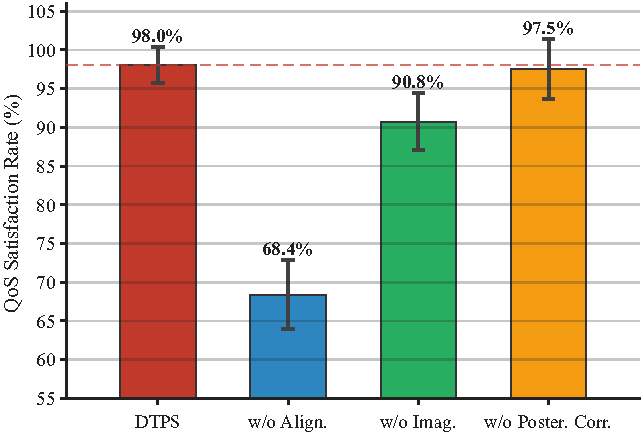
\includegraphics[width=\linewidth]{figures/chapter4/fig9_exp3_ablation_qos.pdf}
        \caption{组件消融}
        \label{fig:ch4_exp_ablation_qos}
    \end{subfigure}
    \hfill
    \begin{subfigure}[t]{0.48\linewidth}
        \centering
        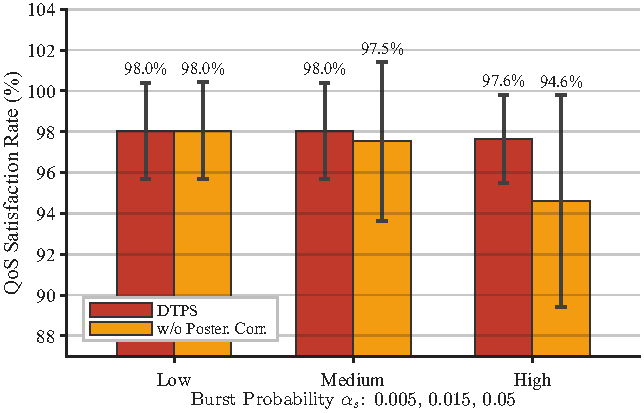
\includegraphics[width=\linewidth]{figures/chapter4/fig9_exp3_ablation_burst.pdf}
        \caption{突发敏感性}
        \label{fig:ch4_exp_ablation_burst}
    \end{subfigure}
    \caption{DTPS 的消融研究}
    \label{fig:ch4_exp_ablation}
\end{figure}

如图~\ref{fig:ch4_exp_ablation_qos} 所示，移除对齐变体带来最大降幅，将 QoS 满足率由 $98.0\%$ 降至 $68.4\%$，这一 $29.6$ 个百分点的下降表明先验—后验对齐对可靠的想象前向推演至关重要。移除想象变体取得 $90.8\%$，较完整 DTPS 低 $7.2$ 个百分点，证实基于想象的策略学习对长视野预测式预算有贡献。移除后验校正变体在中载设置下仅有边际退化，由 $98.0\%$ 降至 $97.5\%$，说明在服务动态相对平滑时所学先验已足够。图~\ref{fig:ch4_exp_ablation_burst} 进一步表明，后验校正在更强突发不确定性下更为重要：在高突发概率（$p_b=0.05$）下，DTPS 维持 $97.6\%$ 的 QoS 满足率，而移除后验校正变体降至 $94.6\%$，其标准差亦升至 $5.2$ 个百分点，相比之下 DTPS 为 $2.2$ 个百分点。总体而言，消融结果表明先验—后验对齐、想象前向推演与在线后验校正分别支撑了可靠的动态学习、长视野策略训练与对突发引起的分布漂移的鲁棒性。

\subsection{固定切片预算下的 MAC 调度}
\label{subsec:ch4_exp_mac}

最后，通过固定切片级带宽与功率预算并在相同资源约束下比较不同调度策略，隔离 MAC 层调度器的贡献。所有切片间隔的带宽与功率预算置为 $W_{s,c}(k)=W_s/|\mathcal C|$、$P_{s,c}(k)=P_s^{\max}/|\mathcal C|$，从而剔除生成式切片资源预留的自适应影响。评估 QCI-Knapsack、Lyapunov-Knapsack 与 Lyapunov-MAC 三种调度器，实验在中载与重载、$p_b=0.015$ 下进行，结果在 10 次独立运行上平均。过载情形被排除于该固定预算实验之外，因为均等切片预算对所有调度器均不足，使不可行性主导对比而掩盖调度层面的差异；过载情形改由启用生成式切片资源预留的完整 DTPS 设置评估。图~\ref{fig:ch4_exp_mac} 显示，QCI-Knapsack 取得最高整体 QoS 满足率，中载下达 $96.9\%$、重载下达 $90.5\%$。Lyapunov-Knapsack 与 Lyapunov-MAC 的对比隔离了 QoS 可行物品构造的效果：重载下 Lyapunov-Knapsack 将 QoS 满足率由 $55.5\%$ 提升至 $78.6\%$，绝对提升 $23.1$ 个百分点。该提升与第~\ref{subsec:ch4_mac}~节的分析一致：在选择前估计最小 RBG—功率需求，可避免将资源分配给当前时隙无法达到 QoS 门限的流。

\begin{figure}[!htp]
    \centering
    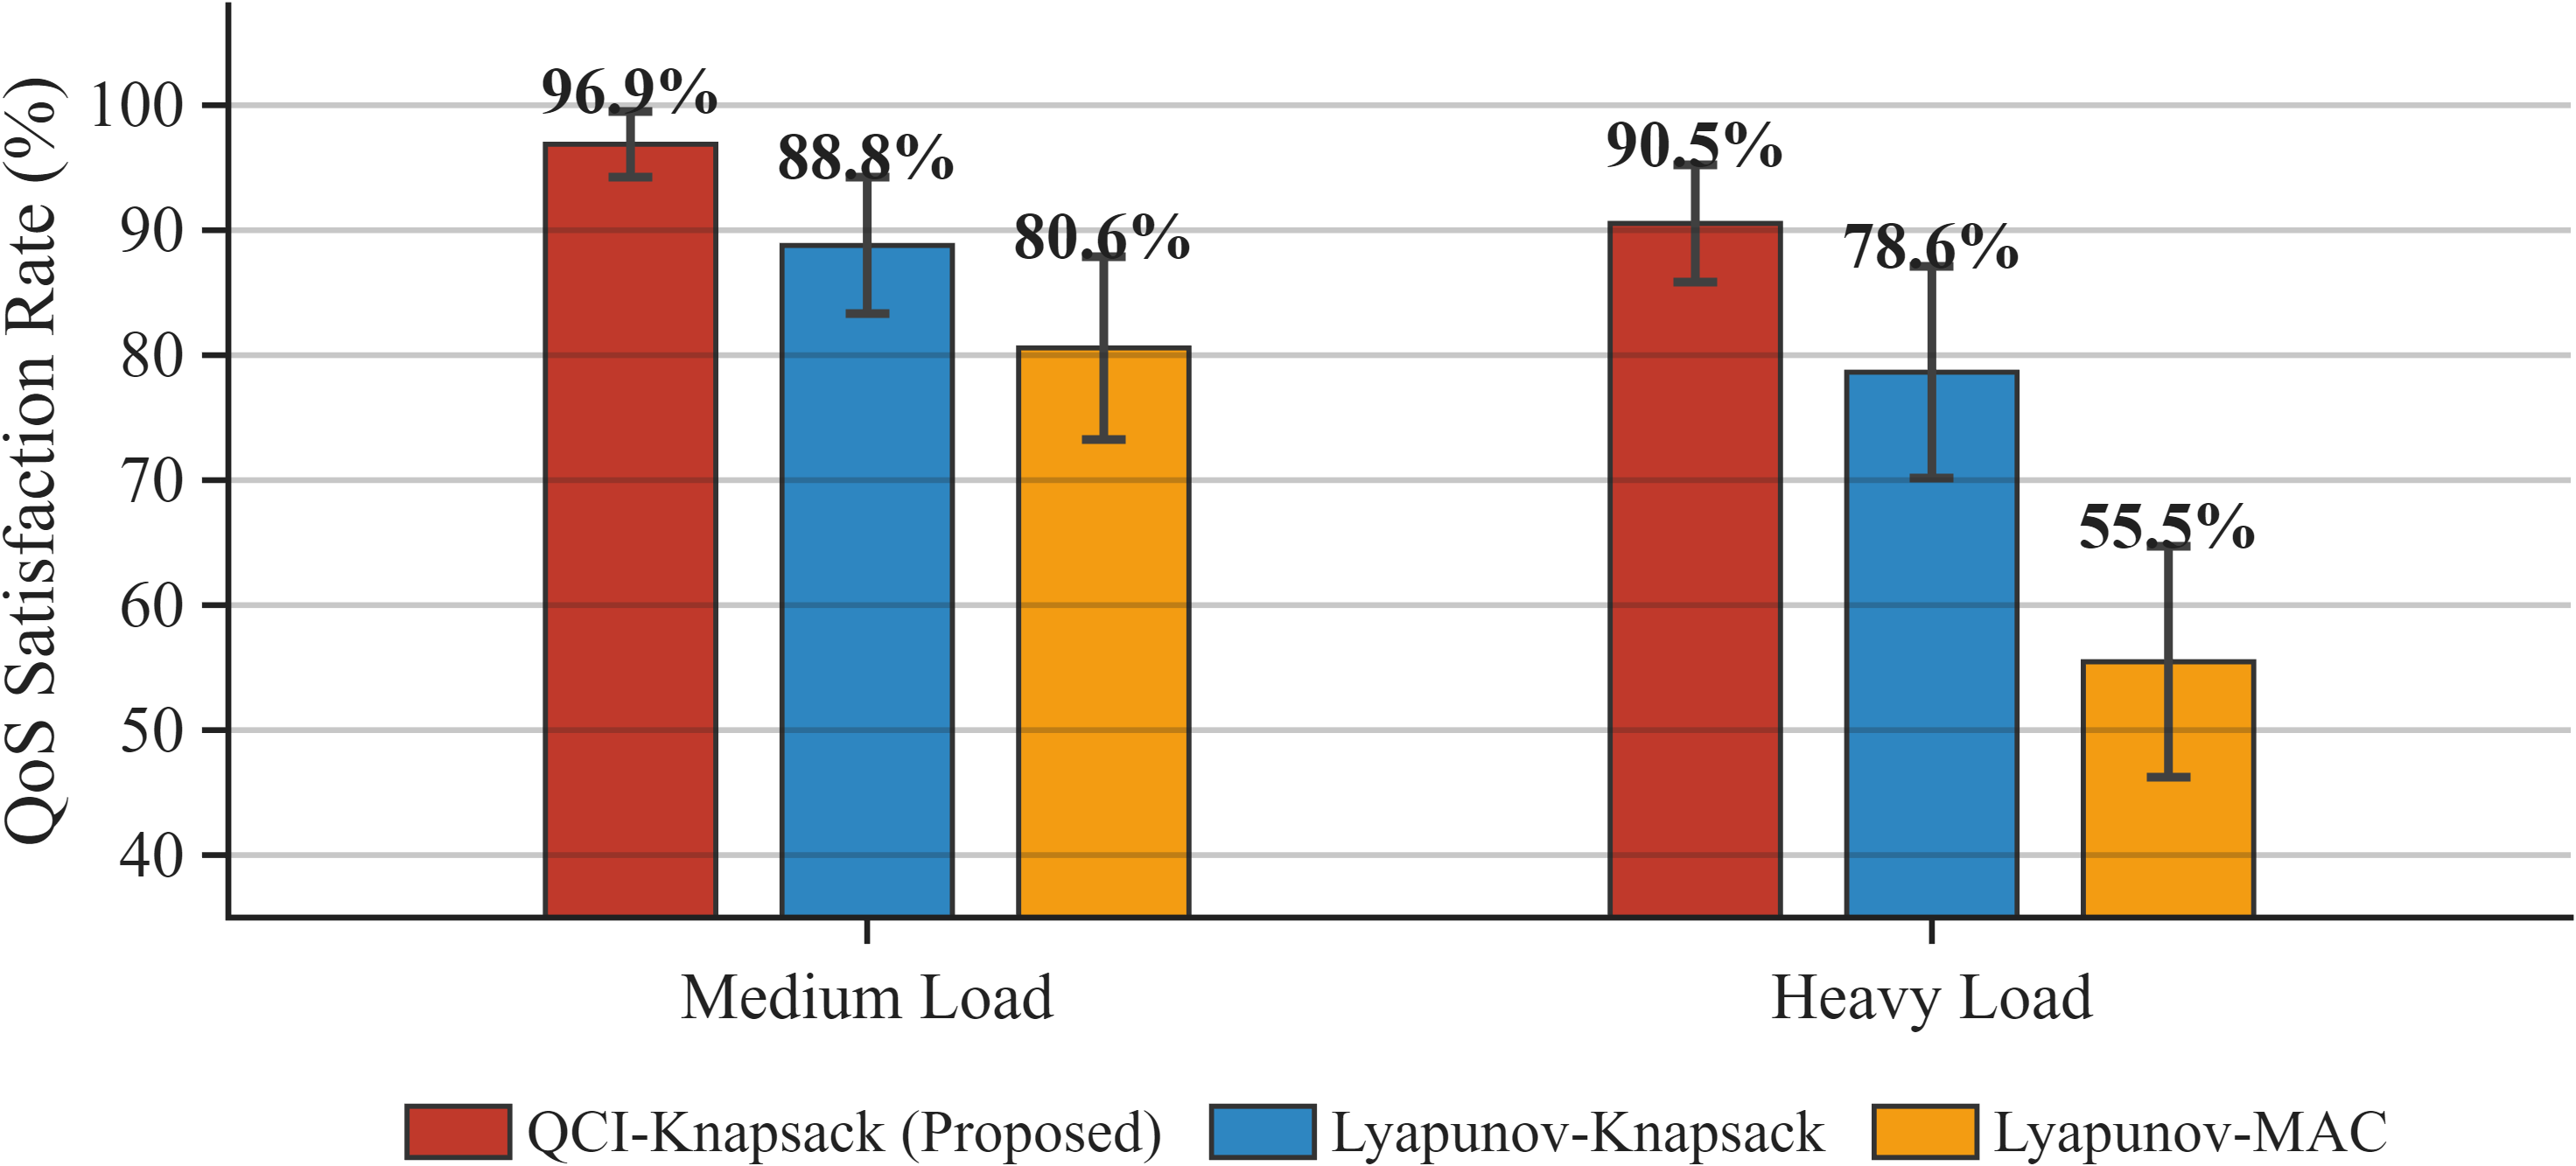
\includegraphics[width=0.72\linewidth]{figures/chapter4/figure10_exp1.png}
    \caption{整体 QoS 满足率}
    \label{fig:ch4_exp_mac}
\end{figure}

\begin{table}[!htp]
\centering
\caption{中载场景下的各切片 QoS 满足率（\%）}
\label{tab:ch4_perslice}
\small
\setlength{\tabcolsep}{6pt}
\renewcommand{\arraystretch}{1.2}
\begin{tabular}{lccc}
\toprule
切片 & QCI-Knap. & Lyap.-Knap. & Lyap.-MAC \\
\midrule
时延敏感型 & $98.53{\pm}3.05$ & $97.20{\pm}4.46$ & $78.25{\pm}8.17$ \\
带宽密集型 & $88.78{\pm}5.99$ & $80.35{\pm}6.44$ & $50.23{\pm}9.68$ \\
\bottomrule
\end{tabular}
\end{table}

QCI-Knapsack 与 Lyapunov-Knapsack 之间的差距进一步反映物品价值设计的作用。QCI-Knapsack 在中载与重载下分别较 Lyapunov-Knapsack 提升 $8.1$ 与 $11.9$ 个百分点，表明随竞争加剧，业务等级感知的选择更为重要。表~\ref{tab:ch4_perslice} 给出中载场景下的各切片视图：在时延敏感型切片中，QCI-Knapsack 与 Lyapunov-Knapsack 取得相近的 $98.53\%$ 与 $97.20\%$ 满足率，而 Lyapunov-MAC 降至 $78.25\%$，说明 QoS 可行性测试是主导因素；在带宽密集型切片中，QCI-Knapsack 达 $88.78\%$，而 Lyapunov-Knapsack 与 Lyapunov-MAC 分别为 $80.35\%$ 与 $50.23\%$，说明当更多候选通过可行性测试时，物品价值设计的影响更为显著。上述结果证实所提 MAC 调度器同时得益于应用级可行性验证与 QCI 感知的背包选择。

\section{本章小结}

本章在纯分布式管控范式下，研究大规模 LEO 卫星接入网（LEO-sRAN）中面向资源使用效率与用户级 QoS 协同保障的接入网切片与跨层无线资源优化。在该场景中，单颗卫星须在受限星上带宽与发射功率下，为已接入用户的异构业务分配资源；切片层粗粒度预算只有经过后续多个 MAC 时隙中的业务到达、信道变化与流级竞争，才最终体现为用户级 QoS 满足效果。由于聚合吞吐并不等价于用户级 QoS 满足，仅以吞吐或队列紧迫度为依据的资源分配难以将有限带宽与功率转化为有效 QoS 收益。为此，本章提出双时间尺度预测调度（DTPS）框架，以带宽与功率预算为跨层接口，将单星本地切片--MAC 资源分配问题分解为切片层的 QoS 可行域保障与 MAC 层的实时调度两个子问题。其中，慢时间尺度的生成式切片资源预留模块通过反馈校正的业务--信道演化预测模型，评估候选预算对长期 QoS 满足率的影响；快时间尺度的 QCI 优先级背包调度模块先估计各候选流满足速率--时延联合门限所需的最小 RBG--功率开销，再在固定切片预算下选取优先级加权的可行业务流集合。

在 Starlink 规模星座上的仿真结果表明，DTPS 在过载业务和突发业务增强条件下均能保持较高的用户级 QoS 满足率，并避免将有限带宽与功率消耗在难以满足 QoS 门限的业务流上。消融结果表明，反馈校正的切片层预测模型、长视野预算评估和在线校正分别支撑了长期 QoS 保障、资源预留稳定性和突发鲁棒性。固定切片预算下的调度对比进一步说明，MAC 层在资源分配前进行 QoS 可行性测试，比单纯依据队列紧迫度或业务优先级调度更为关键。

上述结果表明，在资源受限的 LEO-sRAN 中，资源分配的核心不应是单纯提升聚合吞吐，而应是将有限带宽与功率优先映射为可满足的用户级 QoS 收益。本章面向资源分配环节建立的跨层资源优化机制，与第~\ref{chap:perception}~章的状态感知、第~\ref{chap:handover}~章的接入切换共同覆盖了端到端传输链路的前三个环节；第~\ref{chap:semantic}~章将进一步推进至传输环节，在受限星上载荷与链路条件下研究端到端传输性能与硬件开销之间的协同问题。
